\documentclass[tikz,border=5pt,multi=tikzpicture]{standalone}
\usepackage[UTF8]{ctex}
\usepackage{amsmath}
\usetikzlibrary{arrows.meta,calc}
\definecolor{ink}{HTML}{17365D}
\definecolor{field}{HTML}{287DA8}
\definecolor{force}{HTML}{C56B2A}
\tikzset{every node/.style={font=\small},vec/.style={-{Stealth[length=2mm]},thick},helper/.style={gray,dashed}}
\begin{document}
\begin{tikzpicture}
  \fill[ink] (0,0) circle (1.5pt);
  \draw[vec,force] (0,0)--(-2.8,0) node[left] {$\boldsymbol p_\pi=(-p_0,0,0)$};
  \draw[vec,ink] (0,0)--(1.8,1.25) node[above right] {$\boldsymbol p_+$};
  \draw[vec,field] (0,0)--(1.2,-1.25) node[below right] {$\boldsymbol p_-$};
  \draw[helper] (1.8,1.25)--(3,0)--(1.2,-1.25);
  \draw[vec,gray] (0,0)--(3,0) node[right] {$(p_0,0,0)$};
  \node[below left] at (0,-.12) {$K^+$};
  \node at (.2,1.85) {实验室系：初态静止，总动量为零};
\end{tikzpicture}
\begin{tikzpicture}
  \node at (0,1.8) {双粒子质心系};
  \draw[vec,ink] (0,0)--(.6,.8) node[right] {$\boldsymbol p_* $};
  \draw[vec,field] (0,0)--(-.6,-.8) node[left] {$-\boldsymbol p_* $};
  \fill (0,0) circle (1.2pt);
  \draw[vec,force] (2,0)--(3.2,0) node[midway,above] {$\beta c$};
  \node at (5.2,1.8) {实验室系};
  \draw[helper] (4,0)--(7,0);
  \fill (4,0) circle (1.2pt) node[below] {$O_p$};
  \draw[vec,ink] (4,0)--(6.5,.8) node[right] {$\boldsymbol p_+$};
  \draw[vec,field] (4,0)--(4.9,-.8) node[below] {$\boldsymbol p_-$};
  \draw[<->,gray] (4,-1.3)--(5.7,-1.3) node[midway,below] {$A=p_0/2$};
  \fill (5.7,0) circle (1.2pt);
  \node at (2.6,-2.15) {$p_{+x}=A+au,\quad p_{-x}=A-au,\quad p_{\perp}=bv$};
\end{tikzpicture}
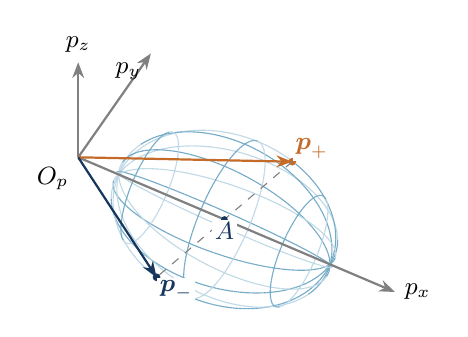
\begin{tikzpicture}
  \draw[field!65,thin] (3.198252,-1.358744)--(3.216607,-1.330685);
\draw[field!65,thin] (3.216607,-1.330685)--(3.233064,-1.301871);
\draw[field!65,thin] (3.233064,-1.301871)--(3.247598,-1.272340);
\draw[field!65,thin] (3.247598,-1.272340)--(3.260189,-1.242135);
\draw[field!65,thin] (3.260189,-1.242135)--(3.270820,-1.211297);
\draw[field!65,thin] (3.270820,-1.211297)--(3.279475,-1.179870);
\draw[field!65,thin] (3.279475,-1.179870)--(3.286143,-1.147897);
\draw[field!65,thin] (3.286143,-1.147897)--(3.290815,-1.115424);
\draw[field!65,thin] (3.290815,-1.115424)--(3.293484,-1.082495);
\draw[field!65,thin] (3.293484,-1.082495)--(3.294146,-1.049157);
\draw[field!30,dashed,thin] (3.294146,-1.049157)--(3.292800,-1.015456);
\draw[field!30,dashed,thin] (3.292800,-1.015456)--(3.289448,-0.981440);
\draw[field!30,dashed,thin] (3.289448,-0.981440)--(3.284095,-0.947154);
\draw[field!30,dashed,thin] (3.284095,-0.947154)--(3.276748,-0.912649);
\draw[field!30,dashed,thin] (3.276748,-0.912649)--(3.267417,-0.877971);
\draw[field!30,dashed,thin] (3.267417,-0.877971)--(3.256117,-0.843170);
\draw[field!30,dashed,thin] (3.256117,-0.843170)--(3.242861,-0.808294);
\draw[field!30,dashed,thin] (3.242861,-0.808294)--(3.227670,-0.773391);
\draw[field!30,dashed,thin] (3.227670,-0.773391)--(3.210563,-0.738510);
\draw[field!30,dashed,thin] (3.210563,-0.738510)--(3.191566,-0.703701);
\draw[field!30,dashed,thin] (3.191566,-0.703701)--(3.170704,-0.669011);
\draw[field!30,dashed,thin] (3.170704,-0.669011)--(3.148007,-0.634489);
\draw[field!30,dashed,thin] (3.148007,-0.634489)--(3.123506,-0.600184);
\draw[field!30,dashed,thin] (3.123506,-0.600184)--(3.097235,-0.566142);
\draw[field!30,dashed,thin] (3.097235,-0.566142)--(3.069232,-0.532413);
\draw[field!30,dashed,thin] (3.069232,-0.532413)--(3.039536,-0.499043);
\draw[field!30,dashed,thin] (3.039536,-0.499043)--(3.008187,-0.466078);
\draw[field!30,dashed,thin] (3.008187,-0.466078)--(2.975230,-0.433565);
\draw[field!30,dashed,thin] (2.975230,-0.433565)--(2.940710,-0.401548);
\draw[field!30,dashed,thin] (2.940710,-0.401548)--(2.904677,-0.370074);
\draw[field!30,dashed,thin] (2.904677,-0.370074)--(2.867179,-0.339185);
\draw[field!30,dashed,thin] (2.867179,-0.339185)--(2.828271,-0.308925);
\draw[field!30,dashed,thin] (2.828271,-0.308925)--(2.788005,-0.279336);
\draw[field!30,dashed,thin] (2.788005,-0.279336)--(2.746438,-0.250460);
\draw[field!30,dashed,thin] (2.746438,-0.250460)--(2.703629,-0.222336);
\draw[field!30,dashed,thin] (2.703629,-0.222336)--(2.659637,-0.195004);
\draw[field!30,dashed,thin] (2.659637,-0.195004)--(2.614523,-0.168503);
\draw[field!30,dashed,thin] (2.614523,-0.168503)--(2.568351,-0.142869);
\draw[field!30,dashed,thin] (2.568351,-0.142869)--(2.521185,-0.118138);
\draw[field!30,dashed,thin] (2.521185,-0.118138)--(2.473091,-0.094344);
\draw[field!30,dashed,thin] (2.473091,-0.094344)--(2.424136,-0.071522);
\draw[field!30,dashed,thin] (2.424136,-0.071522)--(2.374388,-0.049702);
\draw[field!30,dashed,thin] (2.374388,-0.049702)--(2.323918,-0.028915);
\draw[field!30,dashed,thin] (2.323918,-0.028915)--(2.272794,-0.009190);
\draw[field!30,dashed,thin] (2.272794,-0.009190)--(2.221090,0.009445);
\draw[field!30,dashed,thin] (2.221090,0.009445)--(2.168877,0.026964);
\draw[field!30,dashed,thin] (2.168877,0.026964)--(2.116228,0.043342);
\draw[field!30,dashed,thin] (2.116228,0.043342)--(2.063216,0.058558);
\draw[field!30,dashed,thin] (2.063216,0.058558)--(2.009916,0.072589);
\draw[field!30,dashed,thin] (2.009916,0.072589)--(1.956402,0.085416);
\draw[field!30,dashed,thin] (1.956402,0.085416)--(1.902749,0.097021);
\draw[field!30,dashed,thin] (1.902749,0.097021)--(1.849031,0.107389);
\draw[field!30,dashed,thin] (1.849031,0.107389)--(1.795324,0.116503);
\draw[field!30,dashed,thin] (1.795324,0.116503)--(1.741703,0.124352);
\draw[field!30,dashed,thin] (1.741703,0.124352)--(1.688243,0.130925);
\draw[field!30,dashed,thin] (1.688243,0.130925)--(1.635018,0.136212);
\draw[field!30,dashed,thin] (1.635018,0.136212)--(1.582103,0.140207);
\draw[field!30,dashed,thin] (1.582103,0.140207)--(1.529572,0.142903);
\draw[field!30,dashed,thin] (1.529572,0.142903)--(1.477497,0.144297);
\draw[field!30,dashed,thin] (1.477497,0.144297)--(1.425953,0.144386);
\draw[field!30,dashed,thin] (1.425953,0.144386)--(1.375010,0.143172);
\draw[field!30,dashed,thin] (1.375010,0.143172)--(1.324740,0.140654);
\draw[field!30,dashed,thin] (1.324740,0.140654)--(1.275213,0.136838);
\draw[field!30,dashed,thin] (1.275213,0.136838)--(1.226498,0.131728);
\draw[field!30,dashed,thin] (1.226498,0.131728)--(1.178664,0.125331);
\draw[field!30,dashed,thin] (1.178664,0.125331)--(1.131776,0.117657);
\draw[field!30,dashed,thin] (1.131776,0.117657)--(1.085902,0.108716);
\draw[field!30,dashed,thin] (1.085902,0.108716)--(1.041104,0.098520);
\draw[field!30,dashed,thin] (1.041104,0.098520)--(0.997445,0.087084);
\draw[field!30,dashed,thin] (0.997445,0.087084)--(0.954987,0.074424);
\draw[field!30,dashed,thin] (0.954987,0.074424)--(0.913789,0.060557);
\draw[field!30,dashed,thin] (0.913789,0.060557)--(0.873907,0.045503);
\draw[field!30,dashed,thin] (0.873907,0.045503)--(0.835398,0.029283);
\draw[field!30,dashed,thin] (0.835398,0.029283)--(0.798316,0.011919);
\draw[field!30,dashed,thin] (0.798316,0.011919)--(0.762713,-0.006564);
\draw[field!30,dashed,thin] (0.762713,-0.006564)--(0.728637,-0.026141);
\draw[field!30,dashed,thin] (0.728637,-0.026141)--(0.696138,-0.046783);
\draw[field!30,dashed,thin] (0.696138,-0.046783)--(0.665259,-0.068463);
\draw[field!30,dashed,thin] (0.665259,-0.068463)--(0.636045,-0.091150);
\draw[field!30,dashed,thin] (0.636045,-0.091150)--(0.608536,-0.114812);
\draw[field!30,dashed,thin] (0.608536,-0.114812)--(0.582770,-0.139416);
\draw[field!30,dashed,thin] (0.582770,-0.139416)--(0.558784,-0.164928);
\draw[field!30,dashed,thin] (0.558784,-0.164928)--(0.536611,-0.191312);
\draw[field!30,dashed,thin] (0.536611,-0.191312)--(0.516282,-0.218532);
\draw[field!65,thin] (3.198182,-1.358505)--(3.213947,-1.321496);
\draw[field!65,thin] (3.213947,-1.321496)--(3.227815,-1.283743);
\draw[field!65,thin] (3.227815,-1.283743)--(3.239769,-1.245301);
\draw[field!65,thin] (3.239769,-1.245301)--(3.249791,-1.206221);
\draw[field!65,thin] (3.249791,-1.206221)--(3.257866,-1.166559);
\draw[field!65,thin] (3.257866,-1.166559)--(3.263985,-1.126371);
\draw[field!65,thin] (3.263985,-1.126371)--(3.268138,-1.085711);
\draw[field!65,thin] (3.268138,-1.085711)--(3.270320,-1.044638);
\draw[field!65,thin] (3.270320,-1.044638)--(3.270527,-1.003208);
\draw[field!65,thin] (3.270527,-1.003208)--(3.268760,-0.961479);
\draw[field!65,thin] (3.268760,-0.961479)--(3.265020,-0.919510);
\draw[field!65,thin] (3.265020,-0.919510)--(3.259313,-0.877360);
\draw[field!65,thin] (3.259313,-0.877360)--(3.251647,-0.835086);
\draw[field!65,thin] (3.251647,-0.835086)--(3.242032,-0.792749);
\draw[field!65,thin] (3.242032,-0.792749)--(3.230483,-0.750406);
\draw[field!65,thin] (3.230483,-0.750406)--(3.217015,-0.708119);
\draw[field!65,thin] (3.217015,-0.708119)--(3.201646,-0.665944);
\draw[field!65,thin] (3.201646,-0.665944)--(3.184400,-0.623943);
\draw[field!65,thin] (3.184400,-0.623943)--(3.165298,-0.582172);
\draw[field!65,thin] (3.165298,-0.582172)--(3.144369,-0.540691);
\draw[field!65,thin] (3.144369,-0.540691)--(3.121641,-0.499557);
\draw[field!65,thin] (3.121641,-0.499557)--(3.097147,-0.458828);
\draw[field!65,thin] (3.097147,-0.458828)--(3.070920,-0.418560);
\draw[field!65,thin] (3.070920,-0.418560)--(3.042996,-0.378811);
\draw[field!65,thin] (3.042996,-0.378811)--(3.013416,-0.339635);
\draw[field!65,thin] (3.013416,-0.339635)--(2.982221,-0.301087);
\draw[field!65,thin] (2.982221,-0.301087)--(2.949453,-0.263221);
\draw[field!65,thin] (2.949453,-0.263221)--(2.915159,-0.226091);
\draw[field!65,thin] (2.915159,-0.226091)--(2.879386,-0.189747);
\draw[field!65,thin] (2.879386,-0.189747)--(2.842185,-0.154240);
\draw[field!65,thin] (2.842185,-0.154240)--(2.803608,-0.119621);
\draw[field!65,thin] (2.803608,-0.119621)--(2.763708,-0.085937);
\draw[field!30,dashed,thin] (2.763708,-0.085937)--(2.722541,-0.053236);
\draw[field!30,dashed,thin] (2.722541,-0.053236)--(2.680165,-0.021563);
\draw[field!30,dashed,thin] (2.680165,-0.021563)--(2.636639,0.009037);
\draw[field!30,dashed,thin] (2.636639,0.009037)--(2.592023,0.038522);
\draw[field!30,dashed,thin] (2.592023,0.038522)--(2.546380,0.066851);
\draw[field!30,dashed,thin] (2.546380,0.066851)--(2.499774,0.093984);
\draw[field!30,dashed,thin] (2.499774,0.093984)--(2.452270,0.119883);
\draw[field!30,dashed,thin] (2.452270,0.119883)--(2.403934,0.144511);
\draw[field!30,dashed,thin] (2.403934,0.144511)--(2.354834,0.167836);
\draw[field!30,dashed,thin] (2.354834,0.167836)--(2.305038,0.189823);
\draw[field!30,dashed,thin] (2.305038,0.189823)--(2.254616,0.210442);
\draw[field!30,dashed,thin] (2.254616,0.210442)--(2.203638,0.229665);
\draw[field!30,dashed,thin] (2.203638,0.229665)--(2.152175,0.247465);
\draw[field!30,dashed,thin] (2.152175,0.247465)--(2.100300,0.263816);
\draw[field!30,dashed,thin] (2.100300,0.263816)--(2.048085,0.278696);
\draw[field!30,dashed,thin] (2.048085,0.278696)--(1.995602,0.292085);
\draw[field!30,dashed,thin] (1.995602,0.292085)--(1.942925,0.303962);
\draw[field!30,dashed,thin] (1.942925,0.303962)--(1.890128,0.314313);
\draw[field!30,dashed,thin] (1.890128,0.314313)--(1.837285,0.323122);
\draw[field!30,dashed,thin] (1.837285,0.323122)--(1.784468,0.330376);
\draw[field!30,dashed,thin] (1.784468,0.330376)--(1.731753,0.336067);
\draw[field!30,dashed,thin] (1.731753,0.336067)--(1.679212,0.340186);
\draw[field!30,dashed,thin] (1.679212,0.340186)--(1.626919,0.342727);
\draw[field!30,dashed,thin] (1.626919,0.342727)--(1.574948,0.343687);
\draw[field!30,dashed,thin] (1.574948,0.343687)--(1.523369,0.343063);
\draw[field!30,dashed,thin] (1.523369,0.343063)--(1.472257,0.340859);
\draw[field!30,dashed,thin] (1.472257,0.340859)--(1.421681,0.337075);
\draw[field!30,dashed,thin] (1.421681,0.337075)--(1.371714,0.331718);
\draw[field!30,dashed,thin] (1.371714,0.331718)--(1.322423,0.324795);
\draw[field!30,dashed,thin] (1.322423,0.324795)--(1.273880,0.316316);
\draw[field!30,dashed,thin] (1.273880,0.316316)--(1.226150,0.306292);
\draw[field!30,dashed,thin] (1.226150,0.306292)--(1.179301,0.294738);
\draw[field!30,dashed,thin] (1.179301,0.294738)--(1.133398,0.281669);
\draw[field!30,dashed,thin] (1.133398,0.281669)--(1.088506,0.267105);
\draw[field!30,dashed,thin] (1.088506,0.267105)--(1.044687,0.251065);
\draw[field!30,dashed,thin] (1.044687,0.251065)--(1.002002,0.233571);
\draw[field!30,dashed,thin] (1.002002,0.233571)--(0.960511,0.214649);
\draw[field!30,dashed,thin] (0.960511,0.214649)--(0.920272,0.194324);
\draw[field!30,dashed,thin] (0.920272,0.194324)--(0.881341,0.172625);
\draw[field!30,dashed,thin] (0.881341,0.172625)--(0.843772,0.149583);
\draw[field!30,dashed,thin] (0.843772,0.149583)--(0.807619,0.125228);
\draw[field!30,dashed,thin] (0.807619,0.125228)--(0.772931,0.099597);
\draw[field!30,dashed,thin] (0.772931,0.099597)--(0.739756,0.072723);
\draw[field!30,dashed,thin] (0.739756,0.072723)--(0.708142,0.044646);
\draw[field!30,dashed,thin] (0.708142,0.044646)--(0.678133,0.015403);
\draw[field!30,dashed,thin] (0.678133,0.015403)--(0.649769,-0.014963);
\draw[field!30,dashed,thin] (0.649769,-0.014963)--(0.623092,-0.046412);
\draw[field!30,dashed,thin] (0.623092,-0.046412)--(0.598138,-0.078898);
\draw[field!30,dashed,thin] (0.598138,-0.078898)--(0.574942,-0.112377);
\draw[field!30,dashed,thin] (0.574942,-0.112377)--(0.553536,-0.146801);
\draw[field!30,dashed,thin] (0.553536,-0.146801)--(0.533950,-0.182123);
\draw[field!30,dashed,thin] (0.533950,-0.182123)--(0.516213,-0.218293);
\draw[field!65,thin] (3.197993,-1.358527)--(3.206677,-1.322372);
\draw[field!65,thin] (3.206677,-1.322372)--(3.213476,-1.285473);
\draw[field!65,thin] (3.213476,-1.285473)--(3.218380,-1.247880);
\draw[field!65,thin] (3.218380,-1.247880)--(3.221382,-1.209647);
\draw[field!65,thin] (3.221382,-1.209647)--(3.222478,-1.170827);
\draw[field!65,thin] (3.222478,-1.170827)--(3.221666,-1.131475);
\draw[field!65,thin] (3.221666,-1.131475)--(3.218948,-1.091644);
\draw[field!65,thin] (3.218948,-1.091644)--(3.214327,-1.051391);
\draw[field!65,thin] (3.214327,-1.051391)--(3.207809,-1.010772);
\draw[field!65,thin] (3.207809,-1.010772)--(3.199405,-0.969844);
\draw[field!65,thin] (3.199405,-0.969844)--(3.189125,-0.928664);
\draw[field!65,thin] (3.189125,-0.928664)--(3.176984,-0.887289);
\draw[field!65,thin] (3.176984,-0.887289)--(3.162998,-0.845778);
\draw[field!65,thin] (3.162998,-0.845778)--(3.147189,-0.804188);
\draw[field!65,thin] (3.147189,-0.804188)--(3.129576,-0.762577);
\draw[field!65,thin] (3.129576,-0.762577)--(3.110186,-0.721003);
\draw[field!65,thin] (3.110186,-0.721003)--(3.089045,-0.679525);
\draw[field!65,thin] (3.089045,-0.679525)--(3.066183,-0.638201);
\draw[field!65,thin] (3.066183,-0.638201)--(3.041631,-0.597087);
\draw[field!65,thin] (3.041631,-0.597087)--(3.015425,-0.556242);
\draw[field!65,thin] (3.015425,-0.556242)--(2.987599,-0.515723);
\draw[field!65,thin] (2.987599,-0.515723)--(2.958195,-0.475586);
\draw[field!65,thin] (2.958195,-0.475586)--(2.927251,-0.435888);
\draw[field!65,thin] (2.927251,-0.435888)--(2.894813,-0.396683);
\draw[field!65,thin] (2.894813,-0.396683)--(2.860924,-0.358027);
\draw[field!65,thin] (2.860924,-0.358027)--(2.825633,-0.319973);
\draw[field!65,thin] (2.825633,-0.319973)--(2.788989,-0.282575);
\draw[field!65,thin] (2.788989,-0.282575)--(2.751042,-0.245884);
\draw[field!65,thin] (2.751042,-0.245884)--(2.711846,-0.209953);
\draw[field!65,thin] (2.711846,-0.209953)--(2.671456,-0.174832);
\draw[field!65,thin] (2.671456,-0.174832)--(2.629928,-0.140568);
\draw[field!65,thin] (2.629928,-0.140568)--(2.587320,-0.107211);
\draw[field!65,thin] (2.587320,-0.107211)--(2.543691,-0.074807);
\draw[field!65,thin] (2.543691,-0.074807)--(2.499103,-0.043401);
\draw[field!65,thin] (2.499103,-0.043401)--(2.453618,-0.013037);
\draw[field!65,thin] (2.453618,-0.013037)--(2.407298,0.016243);
\draw[field!65,thin] (2.407298,0.016243)--(2.360210,0.044397);
\draw[field!65,thin] (2.360210,0.044397)--(2.312419,0.071387);
\draw[field!65,thin] (2.312419,0.071387)--(2.263991,0.097174);
\draw[field!65,thin] (2.263991,0.097174)--(2.214994,0.121724);
\draw[field!65,thin] (2.214994,0.121724)--(2.165497,0.145000);
\draw[field!65,thin] (2.165497,0.145000)--(2.115569,0.166971);
\draw[field!65,thin] (2.115569,0.166971)--(2.065279,0.187607);
\draw[field!65,thin] (2.065279,0.187607)--(2.014698,0.206878);
\draw[field!65,thin] (2.014698,0.206878)--(1.963896,0.224757);
\draw[field!65,thin] (1.963896,0.224757)--(1.912944,0.241219);
\draw[field!65,thin] (1.912944,0.241219)--(1.861914,0.256243);
\draw[field!65,thin] (1.861914,0.256243)--(1.810877,0.269805);
\draw[field!65,thin] (1.810877,0.269805)--(1.759904,0.281888);
\draw[field!65,thin] (1.759904,0.281888)--(1.709066,0.292475);
\draw[field!65,thin] (1.709066,0.292475)--(1.658435,0.301551);
\draw[field!65,thin] (1.658435,0.301551)--(1.608080,0.309102);
\draw[field!65,thin] (1.608080,0.309102)--(1.558073,0.315120);
\draw[field!65,thin] (1.558073,0.315120)--(1.508483,0.319595);
\draw[field!65,thin] (1.508483,0.319595)--(1.459379,0.322520);
\draw[field!65,thin] (1.459379,0.322520)--(1.410831,0.323893);
\draw[field!65,thin] (1.410831,0.323893)--(1.362905,0.323710);
\draw[field!65,thin] (1.362905,0.323710)--(1.315670,0.321973);
\draw[field!65,thin] (1.315670,0.321973)--(1.269190,0.318683);
\draw[field!65,thin] (1.269190,0.318683)--(1.223530,0.313846);
\draw[field!65,thin] (1.223530,0.313846)--(1.178755,0.307467);
\draw[field!65,thin] (1.178755,0.307467)--(1.134928,0.299557);
\draw[field!65,thin] (1.134928,0.299557)--(1.092108,0.290126);
\draw[field!65,thin] (1.092108,0.290126)--(1.050356,0.279186);
\draw[field!65,thin] (1.050356,0.279186)--(1.009731,0.266754);
\draw[field!65,thin] (1.009731,0.266754)--(0.970289,0.252847);
\draw[field!65,thin] (0.970289,0.252847)--(0.932086,0.237484);
\draw[field!65,thin] (0.932086,0.237484)--(0.895173,0.220687);
\draw[field!65,thin] (0.895173,0.220687)--(0.859604,0.202479);
\draw[field!65,thin] (0.859604,0.202479)--(0.825428,0.182885);
\draw[field!65,thin] (0.825428,0.182885)--(0.792692,0.161933);
\draw[field!30,dashed,thin] (0.792692,0.161933)--(0.761443,0.139653);
\draw[field!30,dashed,thin] (0.761443,0.139653)--(0.731724,0.116075);
\draw[field!30,dashed,thin] (0.731724,0.116075)--(0.703576,0.091232);
\draw[field!30,dashed,thin] (0.703576,0.091232)--(0.677038,0.065159);
\draw[field!30,dashed,thin] (0.677038,0.065159)--(0.652149,0.037892);
\draw[field!30,dashed,thin] (0.652149,0.037892)--(0.628942,0.009470);
\draw[field!30,dashed,thin] (0.628942,0.009470)--(0.607450,-0.020068);
\draw[field!30,dashed,thin] (0.607450,-0.020068)--(0.587703,-0.050680);
\draw[field!30,dashed,thin] (0.587703,-0.050680)--(0.569729,-0.082324);
\draw[field!30,dashed,thin] (0.569729,-0.082324)--(0.553553,-0.114956);
\draw[field!30,dashed,thin] (0.553553,-0.114956)--(0.539197,-0.148530);
\draw[field!30,dashed,thin] (0.539197,-0.148530)--(0.526681,-0.182999);
\draw[field!30,dashed,thin] (0.526681,-0.182999)--(0.516023,-0.218316);
\draw[field!65,thin] (3.197734,-1.358807)--(3.196747,-1.333081);
\draw[field!65,thin] (3.196747,-1.333081)--(3.193889,-1.306595);
\draw[field!65,thin] (3.193889,-1.306595)--(3.189163,-1.279388);
\draw[field!65,thin] (3.189163,-1.279388)--(3.182576,-1.251495);
\draw[field!65,thin] (3.182576,-1.251495)--(3.174136,-1.222958);
\draw[field!65,thin] (3.174136,-1.222958)--(3.163857,-1.193814);
\draw[field!65,thin] (3.163857,-1.193814)--(3.151752,-1.164106);
\draw[field!65,thin] (3.151752,-1.164106)--(3.137838,-1.133874);
\draw[field!65,thin] (3.137838,-1.133874)--(3.122135,-1.103162);
\draw[field!65,thin] (3.122135,-1.103162)--(3.104664,-1.072010);
\draw[field!65,thin] (3.104664,-1.072010)--(3.085450,-1.040464);
\draw[field!65,thin] (3.085450,-1.040464)--(3.064519,-1.008568);
\draw[field!65,thin] (3.064519,-1.008568)--(3.041902,-0.976365);
\draw[field!65,thin] (3.041902,-0.976365)--(3.017629,-0.943901);
\draw[field!65,thin] (3.017629,-0.943901)--(2.991735,-0.911221);
\draw[field!65,thin] (2.991735,-0.911221)--(2.964255,-0.878371);
\draw[field!65,thin] (2.964255,-0.878371)--(2.935229,-0.845397);
\draw[field!65,thin] (2.935229,-0.845397)--(2.904696,-0.812344);
\draw[field!65,thin] (2.904696,-0.812344)--(2.872699,-0.779259);
\draw[field!65,thin] (2.872699,-0.779259)--(2.839283,-0.746189);
\draw[field!65,thin] (2.839283,-0.746189)--(2.804495,-0.713179);
\draw[field!65,thin] (2.804495,-0.713179)--(2.768383,-0.680275);
\draw[field!65,thin] (2.768383,-0.680275)--(2.730997,-0.647523);
\draw[field!65,thin] (2.730997,-0.647523)--(2.692391,-0.614970);
\draw[field!65,thin] (2.692391,-0.614970)--(2.652617,-0.582661);
\draw[field!65,thin] (2.652617,-0.582661)--(2.611731,-0.550640);
\draw[field!65,thin] (2.611731,-0.550640)--(2.569791,-0.518952);
\draw[field!65,thin] (2.569791,-0.518952)--(2.526855,-0.487643);
\draw[field!65,thin] (2.526855,-0.487643)--(2.482983,-0.456754);
\draw[field!65,thin] (2.482983,-0.456754)--(2.438236,-0.426331);
\draw[field!65,thin] (2.438236,-0.426331)--(2.392677,-0.396414);
\draw[field!65,thin] (2.392677,-0.396414)--(2.346369,-0.367047);
\draw[field!65,thin] (2.346369,-0.367047)--(2.299377,-0.338269);
\draw[field!65,thin] (2.299377,-0.338269)--(2.251767,-0.310121);
\draw[field!65,thin] (2.251767,-0.310121)--(2.203606,-0.282643);
\draw[field!65,thin] (2.203606,-0.282643)--(2.154960,-0.255873);
\draw[field!65,thin] (2.154960,-0.255873)--(2.105897,-0.229848);
\draw[field!65,thin] (2.105897,-0.229848)--(2.056486,-0.204604);
\draw[field!65,thin] (2.056486,-0.204604)--(2.006797,-0.180177);
\draw[field!65,thin] (2.006797,-0.180177)--(1.956897,-0.156602);
\draw[field!65,thin] (1.956897,-0.156602)--(1.906858,-0.133910);
\draw[field!65,thin] (1.906858,-0.133910)--(1.856749,-0.112133);
\draw[field!65,thin] (1.856749,-0.112133)--(1.806640,-0.091303);
\draw[field!65,thin] (1.806640,-0.091303)--(1.756601,-0.071448);
\draw[field!65,thin] (1.756601,-0.071448)--(1.706702,-0.052595);
\draw[field!65,thin] (1.706702,-0.052595)--(1.657012,-0.034772);
\draw[field!65,thin] (1.657012,-0.034772)--(1.607601,-0.018002);
\draw[field!65,thin] (1.607601,-0.018002)--(1.558539,-0.002311);
\draw[field!65,thin] (1.558539,-0.002311)--(1.509892,0.012282);
\draw[field!65,thin] (1.509892,0.012282)--(1.461731,0.025755);
\draw[field!65,thin] (1.461731,0.025755)--(1.414121,0.038089);
\draw[field!65,thin] (1.414121,0.038089)--(1.367129,0.049267);
\draw[field!65,thin] (1.367129,0.049267)--(1.320822,0.059274);
\draw[field!65,thin] (1.320822,0.059274)--(1.275263,0.068095);
\draw[field!65,thin] (1.275263,0.068095)--(1.230516,0.075719);
\draw[field!65,thin] (1.230516,0.075719)--(1.186644,0.082135);
\draw[field!65,thin] (1.186644,0.082135)--(1.143707,0.087333);
\draw[field!65,thin] (1.143707,0.087333)--(1.101767,0.091306);
\draw[field!65,thin] (1.101767,0.091306)--(1.060882,0.094049);
\draw[field!65,thin] (1.060882,0.094049)--(1.021108,0.095559);
\draw[field!65,thin] (1.021108,0.095559)--(0.982501,0.095832);
\draw[field!65,thin] (0.982501,0.095832)--(0.945116,0.094868);
\draw[field!65,thin] (0.945116,0.094868)--(0.909003,0.092670);
\draw[field!65,thin] (0.909003,0.092670)--(0.874215,0.089240);
\draw[field!65,thin] (0.874215,0.089240)--(0.840799,0.084582);
\draw[field!65,thin] (0.840799,0.084582)--(0.808802,0.078704);
\draw[field!65,thin] (0.808802,0.078704)--(0.778269,0.071613);
\draw[field!65,thin] (0.778269,0.071613)--(0.749243,0.063319);
\draw[field!65,thin] (0.749243,0.063319)--(0.721763,0.053834);
\draw[field!65,thin] (0.721763,0.053834)--(0.695869,0.043172);
\draw[field!65,thin] (0.695869,0.043172)--(0.671596,0.031346);
\draw[field!65,thin] (0.671596,0.031346)--(0.648979,0.018374);
\draw[field!65,thin] (0.648979,0.018374)--(0.628049,0.004274);
\draw[field!65,thin] (0.628049,0.004274)--(0.608835,-0.010934);
\draw[field!65,thin] (0.608835,-0.010934)--(0.591364,-0.027230);
\draw[field!65,thin] (0.591364,-0.027230)--(0.575660,-0.044591);
\draw[field!65,thin] (0.575660,-0.044591)--(0.561746,-0.062992);
\draw[field!30,dashed,thin] (0.561746,-0.062992)--(0.549641,-0.082407);
\draw[field!30,dashed,thin] (0.549641,-0.082407)--(0.539362,-0.102810);
\draw[field!30,dashed,thin] (0.539362,-0.102810)--(0.530923,-0.124172);
\draw[field!30,dashed,thin] (0.530923,-0.124172)--(0.524335,-0.146464);
\draw[field!30,dashed,thin] (0.524335,-0.146464)--(0.519609,-0.169653);
\draw[field!30,dashed,thin] (0.519609,-0.169653)--(0.516751,-0.193708);
\draw[field!30,dashed,thin] (0.516751,-0.193708)--(0.515764,-0.218595);
\draw[field!65,thin] (3.197475,-1.359267)--(3.186817,-1.350751);
\draw[field!65,thin] (3.186817,-1.350751)--(3.174302,-1.341451);
\draw[field!65,thin] (3.174302,-1.341451)--(3.159945,-1.331380);
\draw[field!65,thin] (3.159945,-1.331380)--(3.143769,-1.320552);
\draw[field!65,thin] (3.143769,-1.320552)--(3.125795,-1.308982);
\draw[field!65,thin] (3.125795,-1.308982)--(3.106048,-1.296686);
\draw[field!65,thin] (3.106048,-1.296686)--(3.084556,-1.283682);
\draw[field!65,thin] (3.084556,-1.283682)--(3.061349,-1.269987);
\draw[field!65,thin] (3.061349,-1.269987)--(3.036460,-1.255620);
\draw[field!65,thin] (3.036460,-1.255620)--(3.009923,-1.240603);
\draw[field!65,thin] (3.009923,-1.240603)--(2.981775,-1.224955);
\draw[field!65,thin] (2.981775,-1.224955)--(2.952055,-1.208699);
\draw[field!65,thin] (2.952055,-1.208699)--(2.920806,-1.191857);
\draw[field!65,thin] (2.920806,-1.191857)--(2.888070,-1.174453);
\draw[field!65,thin] (2.888070,-1.174453)--(2.853894,-1.156511);
\draw[field!65,thin] (2.853894,-1.156511)--(2.818325,-1.138056);
\draw[field!65,thin] (2.818325,-1.138056)--(2.781413,-1.119114);
\draw[field!65,thin] (2.781413,-1.119114)--(2.743209,-1.099712);
\draw[field!65,thin] (2.743209,-1.099712)--(2.703767,-1.079876);
\draw[field!65,thin] (2.703767,-1.079876)--(2.663142,-1.059634);
\draw[field!65,thin] (2.663142,-1.059634)--(2.621390,-1.039015);
\draw[field!65,thin] (2.621390,-1.039015)--(2.578571,-1.018047);
\draw[field!65,thin] (2.578571,-1.018047)--(2.534743,-0.996760);
\draw[field!65,thin] (2.534743,-0.996760)--(2.489968,-0.975183);
\draw[field!65,thin] (2.489968,-0.975183)--(2.444309,-0.953346);
\draw[field!65,thin] (2.444309,-0.953346)--(2.397829,-0.931281);
\draw[field!65,thin] (2.397829,-0.931281)--(2.350593,-0.909017);
\draw[field!65,thin] (2.350593,-0.909017)--(2.302667,-0.886586);
\draw[field!65,thin] (2.302667,-0.886586)--(2.254119,-0.864019);
\draw[field!65,thin] (2.254119,-0.864019)--(2.205015,-0.841349);
\draw[field!65,thin] (2.205015,-0.841349)--(2.155425,-0.818605);
\draw[field!65,thin] (2.155425,-0.818605)--(2.105418,-0.795821);
\draw[field!65,thin] (2.105418,-0.795821)--(2.055064,-0.773027);
\draw[field!65,thin] (2.055064,-0.773027)--(2.004432,-0.750257);
\draw[field!65,thin] (2.004432,-0.750257)--(1.953594,-0.727541);
\draw[field!65,thin] (1.953594,-0.727541)--(1.902621,-0.704912);
\draw[field!65,thin] (1.902621,-0.704912)--(1.851584,-0.682400);
\draw[field!65,thin] (1.851584,-0.682400)--(1.800554,-0.660038);
\draw[field!65,thin] (1.800554,-0.660038)--(1.749602,-0.637857);
\draw[field!65,thin] (1.749602,-0.637857)--(1.698801,-0.615887);
\draw[field!65,thin] (1.698801,-0.615887)--(1.648219,-0.594160);
\draw[field!65,thin] (1.648219,-0.594160)--(1.597930,-0.572705);
\draw[field!65,thin] (1.597930,-0.572705)--(1.548001,-0.551553);
\draw[field!65,thin] (1.548001,-0.551553)--(1.498504,-0.530733);
\draw[field!65,thin] (1.498504,-0.530733)--(1.449507,-0.510274);
\draw[field!65,thin] (1.449507,-0.510274)--(1.401079,-0.490206);
\draw[field!65,thin] (1.401079,-0.490206)--(1.353288,-0.470555);
\draw[field!65,thin] (1.353288,-0.470555)--(1.306200,-0.451349);
\draw[field!65,thin] (1.306200,-0.451349)--(1.259881,-0.432616);
\draw[field!65,thin] (1.259881,-0.432616)--(1.214395,-0.414381);
\draw[field!65,thin] (1.214395,-0.414381)--(1.169807,-0.396670);
\draw[field!65,thin] (1.169807,-0.396670)--(1.126178,-0.379507);
\draw[field!65,thin] (1.126178,-0.379507)--(1.083570,-0.362917);
\draw[field!65,thin] (1.083570,-0.362917)--(1.042042,-0.346922);
\draw[field!65,thin] (1.042042,-0.346922)--(1.001652,-0.331546);
\draw[field!65,thin] (1.001652,-0.331546)--(0.962456,-0.316809);
\draw[field!65,thin] (0.962456,-0.316809)--(0.924509,-0.302732);
\draw[field!65,thin] (0.924509,-0.302732)--(0.887865,-0.289335);
\draw[field!65,thin] (0.887865,-0.289335)--(0.852574,-0.276636);
\draw[field!65,thin] (0.852574,-0.276636)--(0.818685,-0.264654);
\draw[field!65,thin] (0.818685,-0.264654)--(0.786247,-0.253404);
\draw[field!65,thin] (0.786247,-0.253404)--(0.755304,-0.242904);
\draw[field!65,thin] (0.755304,-0.242904)--(0.725899,-0.233166);
\draw[field!65,thin] (0.725899,-0.233166)--(0.698074,-0.224205);
\draw[field!65,thin] (0.698074,-0.224205)--(0.671867,-0.216034);
\draw[field!65,thin] (0.671867,-0.216034)--(0.647315,-0.208664);
\draw[field!65,thin] (0.647315,-0.208664)--(0.624453,-0.202105);
\draw[field!65,thin] (0.624453,-0.202105)--(0.603312,-0.196366);
\draw[field!65,thin] (0.603312,-0.196366)--(0.583922,-0.191455);
\draw[field!65,thin] (0.583922,-0.191455)--(0.566310,-0.187380);
\draw[field!65,thin] (0.566310,-0.187380)--(0.550500,-0.184146);
\draw[field!65,thin] (0.550500,-0.184146)--(0.536515,-0.181756);
\draw[field!65,thin] (0.536515,-0.181756)--(0.524374,-0.180216);
\draw[field!65,thin] (0.524374,-0.180216)--(0.514094,-0.179527);
\draw[field!65,thin] (0.514094,-0.179527)--(0.505689,-0.179689);
\draw[field!65,thin] (0.505689,-0.179689)--(0.499172,-0.180703);
\draw[field!65,thin] (0.499172,-0.180703)--(0.494551,-0.182567);
\draw[field!65,thin] (0.494551,-0.182567)--(0.491832,-0.185279);
\draw[field!30,dashed,thin] (0.491832,-0.185279)--(0.491020,-0.188835);
\draw[field!30,dashed,thin] (0.491020,-0.188835)--(0.492116,-0.193229);
\draw[field!30,dashed,thin] (0.492116,-0.193229)--(0.495118,-0.198456);
\draw[field!30,dashed,thin] (0.495118,-0.198456)--(0.500022,-0.204509);
\draw[field!30,dashed,thin] (0.500022,-0.204509)--(0.506821,-0.211378);
\draw[field!30,dashed,thin] (0.506821,-0.211378)--(0.515506,-0.219055);
\draw[field!65,thin] (3.197286,-1.359786)--(3.179548,-1.370649);
\draw[field!65,thin] (3.179548,-1.370649)--(3.159963,-1.380701);
\draw[field!65,thin] (3.159963,-1.380701)--(3.138557,-1.389927);
\draw[field!65,thin] (3.138557,-1.389927)--(3.115361,-1.398314);
\draw[field!65,thin] (3.115361,-1.398314)--(3.090406,-1.405850);
\draw[field!65,thin] (3.090406,-1.405850)--(3.063729,-1.412525);
\draw[field!65,thin] (3.063729,-1.412525)--(3.035366,-1.418330);
\draw[field!65,thin] (3.035366,-1.418330)--(3.005356,-1.423256);
\draw[field!65,thin] (3.005356,-1.423256)--(2.973742,-1.427297);
\draw[field!65,thin] (2.973742,-1.427297)--(2.940568,-1.430447);
\draw[field!65,thin] (2.940568,-1.430447)--(2.905879,-1.432701);
\draw[field!65,thin] (2.905879,-1.432701)--(2.869726,-1.434057);
\draw[field!65,thin] (2.869726,-1.434057)--(2.832157,-1.434512);
\draw[field!65,thin] (2.832157,-1.434512)--(2.793226,-1.434067);
\draw[field!65,thin] (2.793226,-1.434067)--(2.752987,-1.432720);
\draw[field!65,thin] (2.752987,-1.432720)--(2.711496,-1.430475);
\draw[field!65,thin] (2.711496,-1.430475)--(2.668811,-1.427335);
\draw[field!65,thin] (2.668811,-1.427335)--(2.624992,-1.423303);
\draw[field!65,thin] (2.624992,-1.423303)--(2.580100,-1.418386);
\draw[field!65,thin] (2.580100,-1.418386)--(2.534197,-1.412590);
\draw[field!65,thin] (2.534197,-1.412590)--(2.487348,-1.405924);
\draw[field!65,thin] (2.487348,-1.405924)--(2.439619,-1.398397);
\draw[field!65,thin] (2.439619,-1.398397)--(2.391075,-1.390019);
\draw[field!65,thin] (2.391075,-1.390019)--(2.341785,-1.380802);
\draw[field!65,thin] (2.341785,-1.380802)--(2.291817,-1.370759);
\draw[field!65,thin] (2.291817,-1.370759)--(2.241241,-1.359903);
\draw[field!65,thin] (2.241241,-1.359903)--(2.190129,-1.348251);
\draw[field!65,thin] (2.190129,-1.348251)--(2.138551,-1.335818);
\draw[field!65,thin] (2.138551,-1.335818)--(2.086579,-1.322622);
\draw[field!65,thin] (2.086579,-1.322622)--(2.034286,-1.308681);
\draw[field!65,thin] (2.034286,-1.308681)--(1.981745,-1.294015);
\draw[field!65,thin] (1.981745,-1.294015)--(1.929030,-1.278644);
\draw[field!65,thin] (1.929030,-1.278644)--(1.876213,-1.262589);
\draw[field!65,thin] (1.876213,-1.262589)--(1.823370,-1.245874);
\draw[field!65,thin] (1.823370,-1.245874)--(1.770573,-1.228521);
\draw[field!65,thin] (1.770573,-1.228521)--(1.717896,-1.210554);
\draw[field!65,thin] (1.717896,-1.210554)--(1.665414,-1.191999);
\draw[field!65,thin] (1.665414,-1.191999)--(1.613198,-1.172882);
\draw[field!65,thin] (1.613198,-1.172882)--(1.561323,-1.153229);
\draw[field!65,thin] (1.561323,-1.153229)--(1.509861,-1.133068);
\draw[field!65,thin] (1.509861,-1.133068)--(1.458883,-1.112427);
\draw[field!65,thin] (1.458883,-1.112427)--(1.408460,-1.091334);
\draw[field!65,thin] (1.408460,-1.091334)--(1.358664,-1.069820);
\draw[field!65,thin] (1.358664,-1.069820)--(1.309564,-1.047914);
\draw[field!65,thin] (1.309564,-1.047914)--(1.261228,-1.025647);
\draw[field!65,thin] (1.261228,-1.025647)--(1.213724,-1.003049);
\draw[field!65,thin] (1.213724,-1.003049)--(1.167118,-0.980154);
\draw[field!65,thin] (1.167118,-0.980154)--(1.121475,-0.956992);
\draw[field!65,thin] (1.121475,-0.956992)--(1.076860,-0.933596);
\draw[field!65,thin] (1.076860,-0.933596)--(1.033333,-0.909998);
\draw[field!65,thin] (1.033333,-0.909998)--(0.990957,-0.886232);
\draw[field!65,thin] (0.990957,-0.886232)--(0.949790,-0.862330);
\draw[field!65,thin] (0.949790,-0.862330)--(0.909890,-0.838327);
\draw[field!65,thin] (0.909890,-0.838327)--(0.871313,-0.814255);
\draw[field!65,thin] (0.871313,-0.814255)--(0.834112,-0.790149);
\draw[field!65,thin] (0.834112,-0.790149)--(0.798339,-0.766041);
\draw[field!65,thin] (0.798339,-0.766041)--(0.764045,-0.741966);
\draw[field!65,thin] (0.764045,-0.741966)--(0.731278,-0.717958);
\draw[field!65,thin] (0.731278,-0.717958)--(0.700082,-0.694049);
\draw[field!65,thin] (0.700082,-0.694049)--(0.670502,-0.670273);
\draw[field!65,thin] (0.670502,-0.670273)--(0.642579,-0.646664);
\draw[field!65,thin] (0.642579,-0.646664)--(0.616352,-0.623254);
\draw[field!65,thin] (0.616352,-0.623254)--(0.591857,-0.600075);
\draw[field!65,thin] (0.591857,-0.600075)--(0.569129,-0.577162);
\draw[field!65,thin] (0.569129,-0.577162)--(0.548200,-0.554545);
\draw[field!65,thin] (0.548200,-0.554545)--(0.529099,-0.532256);
\draw[field!65,thin] (0.529099,-0.532256)--(0.511852,-0.510325);
\draw[field!65,thin] (0.511852,-0.510325)--(0.496484,-0.488785);
\draw[field!65,thin] (0.496484,-0.488785)--(0.483015,-0.467665);
\draw[field!65,thin] (0.483015,-0.467665)--(0.471466,-0.446994);
\draw[field!65,thin] (0.471466,-0.446994)--(0.461851,-0.426801);
\draw[field!65,thin] (0.461851,-0.426801)--(0.454185,-0.407115);
\draw[field!65,thin] (0.454185,-0.407115)--(0.448478,-0.387963);
\draw[field!65,thin] (0.448478,-0.387963)--(0.444738,-0.369371);
\draw[field!65,thin] (0.444738,-0.369371)--(0.442971,-0.351366);
\draw[field!65,thin] (0.442971,-0.351366)--(0.443178,-0.333973);
\draw[field!65,thin] (0.443178,-0.333973)--(0.445360,-0.317216);
\draw[field!65,thin] (0.445360,-0.317216)--(0.449513,-0.301118);
\draw[field!30,dashed,thin] (0.449513,-0.301118)--(0.455632,-0.285703);
\draw[field!30,dashed,thin] (0.455632,-0.285703)--(0.463708,-0.270991);
\draw[field!30,dashed,thin] (0.463708,-0.270991)--(0.473729,-0.257003);
\draw[field!30,dashed,thin] (0.473729,-0.257003)--(0.485683,-0.243759);
\draw[field!30,dashed,thin] (0.485683,-0.243759)--(0.499552,-0.231276);
\draw[field!30,dashed,thin] (0.499552,-0.231276)--(0.515316,-0.219574);
\draw[field!65,thin] (3.197216,-1.360223)--(3.176887,-1.387443);
\draw[field!65,thin] (3.176887,-1.387443)--(3.154714,-1.413828);
\draw[field!65,thin] (3.154714,-1.413828)--(3.130728,-1.439340);
\draw[field!65,thin] (3.130728,-1.439340)--(3.104962,-1.463944);
\draw[field!65,thin] (3.104962,-1.463944)--(3.077453,-1.487606);
\draw[field!65,thin] (3.077453,-1.487606)--(3.048239,-1.510293);
\draw[field!65,thin] (3.048239,-1.510293)--(3.017360,-1.531973);
\draw[field!65,thin] (3.017360,-1.531973)--(2.984861,-1.552615);
\draw[field!65,thin] (2.984861,-1.552615)--(2.950785,-1.572192);
\draw[field!65,thin] (2.950785,-1.572192)--(2.915182,-1.590675);
\draw[field!65,thin] (2.915182,-1.590675)--(2.878100,-1.608038);
\draw[field!65,thin] (2.878100,-1.608038)--(2.839591,-1.624258);
\draw[field!65,thin] (2.839591,-1.624258)--(2.799710,-1.639312);
\draw[field!65,thin] (2.799710,-1.639312)--(2.758511,-1.653179);
\draw[field!65,thin] (2.758511,-1.653179)--(2.716053,-1.665840);
\draw[field!65,thin] (2.716053,-1.665840)--(2.672394,-1.677276);
\draw[field!65,thin] (2.672394,-1.677276)--(2.627596,-1.687471);
\draw[field!65,thin] (2.627596,-1.687471)--(2.581722,-1.696413);
\draw[field!65,thin] (2.581722,-1.696413)--(2.534835,-1.704087);
\draw[field!65,thin] (2.534835,-1.704087)--(2.487000,-1.710484);
\draw[field!65,thin] (2.487000,-1.710484)--(2.438286,-1.715594);
\draw[field!65,thin] (2.438286,-1.715594)--(2.388759,-1.719410);
\draw[field!65,thin] (2.388759,-1.719410)--(2.338489,-1.721927);
\draw[field!65,thin] (2.338489,-1.721927)--(2.287546,-1.723142);
\draw[field!65,thin] (2.287546,-1.723142)--(2.236001,-1.723052);
\draw[field!65,thin] (2.236001,-1.723052)--(2.183926,-1.721659);
\draw[field!65,thin] (2.183926,-1.721659)--(2.131395,-1.718963);
\draw[field!65,thin] (2.131395,-1.718963)--(2.078480,-1.714968);
\draw[field!65,thin] (2.078480,-1.714968)--(2.025255,-1.709681);
\draw[field!65,thin] (2.025255,-1.709681)--(1.971795,-1.703108);
\draw[field!65,thin] (1.971795,-1.703108)--(1.918174,-1.695259);
\draw[field!65,thin] (1.918174,-1.695259)--(1.864467,-1.686144);
\draw[field!65,thin] (1.864467,-1.686144)--(1.810750,-1.675777);
\draw[field!65,thin] (1.810750,-1.675777)--(1.757097,-1.664172);
\draw[field!65,thin] (1.757097,-1.664172)--(1.703582,-1.651345);
\draw[field!65,thin] (1.703582,-1.651345)--(1.650282,-1.637314);
\draw[field!65,thin] (1.650282,-1.637314)--(1.597271,-1.622098);
\draw[field!65,thin] (1.597271,-1.622098)--(1.544621,-1.605719);
\draw[field!65,thin] (1.544621,-1.605719)--(1.492408,-1.588200);
\draw[field!65,thin] (1.492408,-1.588200)--(1.440704,-1.569565);
\draw[field!65,thin] (1.440704,-1.569565)--(1.389581,-1.549841);
\draw[field!65,thin] (1.389581,-1.549841)--(1.339110,-1.529054);
\draw[field!65,thin] (1.339110,-1.529054)--(1.289362,-1.507234);
\draw[field!65,thin] (1.289362,-1.507234)--(1.240407,-1.484411);
\draw[field!65,thin] (1.240407,-1.484411)--(1.192313,-1.460618);
\draw[field!65,thin] (1.192313,-1.460618)--(1.145147,-1.435887);
\draw[field!65,thin] (1.145147,-1.435887)--(1.098975,-1.410253);
\draw[field!65,thin] (1.098975,-1.410253)--(1.053861,-1.383751);
\draw[field!65,thin] (1.053861,-1.383751)--(1.009869,-1.356420);
\draw[field!65,thin] (1.009869,-1.356420)--(0.967060,-1.328296);
\draw[field!65,thin] (0.967060,-1.328296)--(0.925493,-1.299419);
\draw[field!65,thin] (0.925493,-1.299419)--(0.885228,-1.269831);
\draw[field!65,thin] (0.885228,-1.269831)--(0.846319,-1.239571);
\draw[field!65,thin] (0.846319,-1.239571)--(0.808822,-1.208682);
\draw[field!65,thin] (0.808822,-1.208682)--(0.772788,-1.177207);
\draw[field!65,thin] (0.772788,-1.177207)--(0.738269,-1.145191);
\draw[field!65,thin] (0.738269,-1.145191)--(0.705311,-1.112678);
\draw[field!65,thin] (0.705311,-1.112678)--(0.673963,-1.079713);
\draw[field!65,thin] (0.673963,-1.079713)--(0.644266,-1.046343);
\draw[field!65,thin] (0.644266,-1.046343)--(0.616263,-1.012613);
\draw[field!65,thin] (0.616263,-1.012613)--(0.589993,-0.978572);
\draw[field!65,thin] (0.589993,-0.978572)--(0.565492,-0.944267);
\draw[field!65,thin] (0.565492,-0.944267)--(0.542794,-0.909745);
\draw[field!65,thin] (0.542794,-0.909745)--(0.521932,-0.875055);
\draw[field!65,thin] (0.521932,-0.875055)--(0.502935,-0.840246);
\draw[field!65,thin] (0.502935,-0.840246)--(0.485828,-0.805365);
\draw[field!65,thin] (0.485828,-0.805365)--(0.470637,-0.770462);
\draw[field!65,thin] (0.470637,-0.770462)--(0.457382,-0.735586);
\draw[field!65,thin] (0.457382,-0.735586)--(0.446081,-0.700784);
\draw[field!65,thin] (0.446081,-0.700784)--(0.436751,-0.666107);
\draw[field!65,thin] (0.436751,-0.666107)--(0.429404,-0.631601);
\draw[field!65,thin] (0.429404,-0.631601)--(0.424051,-0.597316);
\draw[field!65,thin] (0.424051,-0.597316)--(0.420699,-0.563299);
\draw[field!65,thin] (0.420699,-0.563299)--(0.419353,-0.529598);
\draw[field!30,dashed,thin] (0.419353,-0.529598)--(0.420014,-0.496260);
\draw[field!30,dashed,thin] (0.420014,-0.496260)--(0.422683,-0.463332);
\draw[field!30,dashed,thin] (0.422683,-0.463332)--(0.427355,-0.430858);
\draw[field!30,dashed,thin] (0.427355,-0.430858)--(0.434023,-0.398886);
\draw[field!30,dashed,thin] (0.434023,-0.398886)--(0.442679,-0.367459);
\draw[field!30,dashed,thin] (0.442679,-0.367459)--(0.453310,-0.336621);
\draw[field!30,dashed,thin] (0.453310,-0.336621)--(0.465901,-0.306416);
\draw[field!30,dashed,thin] (0.465901,-0.306416)--(0.480435,-0.276885);
\draw[field!30,dashed,thin] (0.480435,-0.276885)--(0.496891,-0.248070);
\draw[field!30,dashed,thin] (0.496891,-0.248070)--(0.515247,-0.220012);
\draw[field!65,thin] (3.197286,-1.360463)--(3.179548,-1.396633);
\draw[field!65,thin] (3.179548,-1.396633)--(3.159963,-1.431955);
\draw[field!65,thin] (3.159963,-1.431955)--(3.138557,-1.466379);
\draw[field!65,thin] (3.138557,-1.466379)--(3.115361,-1.499858);
\draw[field!65,thin] (3.115361,-1.499858)--(3.090406,-1.532344);
\draw[field!65,thin] (3.090406,-1.532344)--(3.063729,-1.563792);
\draw[field!65,thin] (3.063729,-1.563792)--(3.035366,-1.594159);
\draw[field!65,thin] (3.035366,-1.594159)--(3.005356,-1.623402);
\draw[field!65,thin] (3.005356,-1.623402)--(2.973742,-1.651479);
\draw[field!65,thin] (2.973742,-1.651479)--(2.940568,-1.678353);
\draw[field!65,thin] (2.940568,-1.678353)--(2.905879,-1.703984);
\draw[field!65,thin] (2.905879,-1.703984)--(2.869726,-1.728338);
\draw[field!65,thin] (2.869726,-1.728338)--(2.832157,-1.751381);
\draw[field!65,thin] (2.832157,-1.751381)--(2.793226,-1.773080);
\draw[field!65,thin] (2.793226,-1.773080)--(2.752987,-1.793405);
\draw[field!65,thin] (2.752987,-1.793405)--(2.711496,-1.812327);
\draw[field!65,thin] (2.711496,-1.812327)--(2.668811,-1.829820);
\draw[field!65,thin] (2.668811,-1.829820)--(2.624992,-1.845861);
\draw[field!65,thin] (2.624992,-1.845861)--(2.580100,-1.860425);
\draw[field!65,thin] (2.580100,-1.860425)--(2.534197,-1.873494);
\draw[field!65,thin] (2.534197,-1.873494)--(2.487348,-1.885048);
\draw[field!65,thin] (2.487348,-1.885048)--(2.439619,-1.895072);
\draw[field!65,thin] (2.439619,-1.895072)--(2.391075,-1.903551);
\draw[field!65,thin] (2.391075,-1.903551)--(2.341785,-1.910474);
\draw[field!65,thin] (2.341785,-1.910474)--(2.291817,-1.915831);
\draw[field!65,thin] (2.291817,-1.915831)--(2.241241,-1.919614);
\draw[field!65,thin] (2.241241,-1.919614)--(2.190129,-1.921819);
\draw[field!65,thin] (2.190129,-1.921819)--(2.138551,-1.922442);
\draw[field!65,thin] (2.138551,-1.922442)--(2.086579,-1.921483);
\draw[field!65,thin] (2.086579,-1.921483)--(2.034286,-1.918942);
\draw[field!65,thin] (2.034286,-1.918942)--(1.981745,-1.914823);
\draw[field!65,thin] (1.981745,-1.914823)--(1.929030,-1.909132);
\draw[field!65,thin] (1.929030,-1.909132)--(1.876213,-1.901877);
\draw[field!65,thin] (1.876213,-1.901877)--(1.823370,-1.893068);
\draw[field!65,thin] (1.823370,-1.893068)--(1.770573,-1.882718);
\draw[field!65,thin] (1.770573,-1.882718)--(1.717896,-1.870840);
\draw[field!65,thin] (1.717896,-1.870840)--(1.665414,-1.857452);
\draw[field!65,thin] (1.665414,-1.857452)--(1.613198,-1.842572);
\draw[field!65,thin] (1.613198,-1.842572)--(1.561323,-1.826221);
\draw[field!65,thin] (1.561323,-1.826221)--(1.509861,-1.808421);
\draw[field!65,thin] (1.509861,-1.808421)--(1.458883,-1.789198);
\draw[field!65,thin] (1.458883,-1.789198)--(1.408460,-1.768579);
\draw[field!65,thin] (1.408460,-1.768579)--(1.358664,-1.746591);
\draw[field!65,thin] (1.358664,-1.746591)--(1.309564,-1.723267);
\draw[field!65,thin] (1.309564,-1.723267)--(1.261228,-1.698638);
\draw[field!65,thin] (1.261228,-1.698638)--(1.213724,-1.672739);
\draw[field!65,thin] (1.213724,-1.672739)--(1.167118,-1.645607);
\draw[field!65,thin] (1.167118,-1.645607)--(1.121475,-1.617278);
\draw[field!65,thin] (1.121475,-1.617278)--(1.076860,-1.587793);
\draw[field!65,thin] (1.076860,-1.587793)--(1.033333,-1.557192);
\draw[field!65,thin] (1.033333,-1.557192)--(0.990957,-1.525520);
\draw[field!65,thin] (0.990957,-1.525520)--(0.949790,-1.492818);
\draw[field!30,dashed,thin] (0.949790,-1.492818)--(0.909890,-1.459135);
\draw[field!30,dashed,thin] (0.909890,-1.459135)--(0.871313,-1.424516);
\draw[field!30,dashed,thin] (0.871313,-1.424516)--(0.834112,-1.389009);
\draw[field!30,dashed,thin] (0.834112,-1.389009)--(0.798339,-1.352665);
\draw[field!30,dashed,thin] (0.798339,-1.352665)--(0.764045,-1.315534);
\draw[field!30,dashed,thin] (0.764045,-1.315534)--(0.731278,-1.277669);
\draw[field!30,dashed,thin] (0.731278,-1.277669)--(0.700082,-1.239121);
\draw[field!30,dashed,thin] (0.700082,-1.239121)--(0.670502,-1.199945);
\draw[field!30,dashed,thin] (0.670502,-1.199945)--(0.642579,-1.160196);
\draw[field!30,dashed,thin] (0.642579,-1.160196)--(0.616352,-1.119928);
\draw[field!30,dashed,thin] (0.616352,-1.119928)--(0.591857,-1.079199);
\draw[field!30,dashed,thin] (0.591857,-1.079199)--(0.569129,-1.038065);
\draw[field!30,dashed,thin] (0.569129,-1.038065)--(0.548200,-0.996584);
\draw[field!30,dashed,thin] (0.548200,-0.996584)--(0.529099,-0.954813);
\draw[field!30,dashed,thin] (0.529099,-0.954813)--(0.511852,-0.912811);
\draw[field!30,dashed,thin] (0.511852,-0.912811)--(0.496484,-0.870637);
\draw[field!30,dashed,thin] (0.496484,-0.870637)--(0.483015,-0.828349);
\draw[field!30,dashed,thin] (0.483015,-0.828349)--(0.471466,-0.786007);
\draw[field!30,dashed,thin] (0.471466,-0.786007)--(0.461851,-0.743670);
\draw[field!30,dashed,thin] (0.461851,-0.743670)--(0.454185,-0.701396);
\draw[field!30,dashed,thin] (0.454185,-0.701396)--(0.448478,-0.659245);
\draw[field!30,dashed,thin] (0.448478,-0.659245)--(0.444738,-0.617276);
\draw[field!30,dashed,thin] (0.444738,-0.617276)--(0.442971,-0.575548);
\draw[field!30,dashed,thin] (0.442971,-0.575548)--(0.443178,-0.534118);
\draw[field!30,dashed,thin] (0.443178,-0.534118)--(0.445360,-0.493045);
\draw[field!30,dashed,thin] (0.445360,-0.493045)--(0.449513,-0.452385);
\draw[field!30,dashed,thin] (0.449513,-0.452385)--(0.455632,-0.412196);
\draw[field!30,dashed,thin] (0.455632,-0.412196)--(0.463708,-0.372535);
\draw[field!30,dashed,thin] (0.463708,-0.372535)--(0.473729,-0.333455);
\draw[field!30,dashed,thin] (0.473729,-0.333455)--(0.485683,-0.295012);
\draw[field!30,dashed,thin] (0.485683,-0.295012)--(0.499552,-0.257260);
\draw[field!30,dashed,thin] (0.499552,-0.257260)--(0.515316,-0.220251);
\draw[field!65,thin] (3.197475,-1.360440)--(3.186817,-1.395756);
\draw[field!65,thin] (3.186817,-1.395756)--(3.174302,-1.430225);
\draw[field!65,thin] (3.174302,-1.430225)--(3.159945,-1.463799);
\draw[field!65,thin] (3.159945,-1.463799)--(3.143769,-1.496431);
\draw[field!65,thin] (3.143769,-1.496431)--(3.125795,-1.528076);
\draw[field!65,thin] (3.125795,-1.528076)--(3.106048,-1.558688);
\draw[field!65,thin] (3.106048,-1.558688)--(3.084556,-1.588226);
\draw[field!65,thin] (3.084556,-1.588226)--(3.061349,-1.616648);
\draw[field!65,thin] (3.061349,-1.616648)--(3.036460,-1.643915);
\draw[field!65,thin] (3.036460,-1.643915)--(3.009923,-1.669988);
\draw[field!65,thin] (3.009923,-1.669988)--(2.981775,-1.694831);
\draw[field!65,thin] (2.981775,-1.694831)--(2.952055,-1.718409);
\draw[field!65,thin] (2.952055,-1.718409)--(2.920806,-1.740689);
\draw[field!30,dashed,thin] (2.920806,-1.740689)--(2.888070,-1.761641);
\draw[field!30,dashed,thin] (2.888070,-1.761641)--(2.853894,-1.781234);
\draw[field!30,dashed,thin] (2.853894,-1.781234)--(2.818325,-1.799443);
\draw[field!30,dashed,thin] (2.818325,-1.799443)--(2.781413,-1.816240);
\draw[field!30,dashed,thin] (2.781413,-1.816240)--(2.743209,-1.831603);
\draw[field!30,dashed,thin] (2.743209,-1.831603)--(2.703767,-1.845510);
\draw[field!30,dashed,thin] (2.703767,-1.845510)--(2.663142,-1.857942);
\draw[field!30,dashed,thin] (2.663142,-1.857942)--(2.621390,-1.868881);
\draw[field!30,dashed,thin] (2.621390,-1.868881)--(2.578571,-1.878313);
\draw[field!30,dashed,thin] (2.578571,-1.878313)--(2.534743,-1.886223);
\draw[field!30,dashed,thin] (2.534743,-1.886223)--(2.489968,-1.892602);
\draw[field!30,dashed,thin] (2.489968,-1.892602)--(2.444309,-1.897439);
\draw[field!30,dashed,thin] (2.444309,-1.897439)--(2.397829,-1.900729);
\draw[field!30,dashed,thin] (2.397829,-1.900729)--(2.350593,-1.902466);
\draw[field!30,dashed,thin] (2.350593,-1.902466)--(2.302667,-1.902648);
\draw[field!30,dashed,thin] (2.302667,-1.902648)--(2.254119,-1.901276);
\draw[field!30,dashed,thin] (2.254119,-1.901276)--(2.205015,-1.898350);
\draw[field!30,dashed,thin] (2.205015,-1.898350)--(2.155425,-1.893876);
\draw[field!30,dashed,thin] (2.155425,-1.893876)--(2.105418,-1.887858);
\draw[field!30,dashed,thin] (2.105418,-1.887858)--(2.055064,-1.880306);
\draw[field!30,dashed,thin] (2.055064,-1.880306)--(2.004432,-1.871231);
\draw[field!30,dashed,thin] (2.004432,-1.871231)--(1.953594,-1.860644);
\draw[field!30,dashed,thin] (1.953594,-1.860644)--(1.902621,-1.848561);
\draw[field!30,dashed,thin] (1.902621,-1.848561)--(1.851584,-1.834998);
\draw[field!30,dashed,thin] (1.851584,-1.834998)--(1.800554,-1.819975);
\draw[field!30,dashed,thin] (1.800554,-1.819975)--(1.749602,-1.803512);
\draw[field!30,dashed,thin] (1.749602,-1.803512)--(1.698801,-1.785633);
\draw[field!30,dashed,thin] (1.698801,-1.785633)--(1.648219,-1.766362);
\draw[field!30,dashed,thin] (1.648219,-1.766362)--(1.597930,-1.745727);
\draw[field!30,dashed,thin] (1.597930,-1.745727)--(1.548001,-1.723756);
\draw[field!30,dashed,thin] (1.548001,-1.723756)--(1.498504,-1.700479);
\draw[field!30,dashed,thin] (1.498504,-1.700479)--(1.449507,-1.675930);
\draw[field!30,dashed,thin] (1.449507,-1.675930)--(1.401079,-1.650143);
\draw[field!30,dashed,thin] (1.401079,-1.650143)--(1.353288,-1.623153);
\draw[field!30,dashed,thin] (1.353288,-1.623153)--(1.306200,-1.594999);
\draw[field!30,dashed,thin] (1.306200,-1.594999)--(1.259881,-1.565719);
\draw[field!30,dashed,thin] (1.259881,-1.565719)--(1.214395,-1.535355);
\draw[field!30,dashed,thin] (1.214395,-1.535355)--(1.169807,-1.503949);
\draw[field!30,dashed,thin] (1.169807,-1.503949)--(1.126178,-1.471544);
\draw[field!30,dashed,thin] (1.126178,-1.471544)--(1.083570,-1.438187);
\draw[field!30,dashed,thin] (1.083570,-1.438187)--(1.042042,-1.403924);
\draw[field!30,dashed,thin] (1.042042,-1.403924)--(1.001652,-1.368802);
\draw[field!30,dashed,thin] (1.001652,-1.368802)--(0.962456,-1.332871);
\draw[field!30,dashed,thin] (0.962456,-1.332871)--(0.924509,-1.296181);
\draw[field!30,dashed,thin] (0.924509,-1.296181)--(0.887865,-1.258783);
\draw[field!30,dashed,thin] (0.887865,-1.258783)--(0.852574,-1.220729);
\draw[field!30,dashed,thin] (0.852574,-1.220729)--(0.818685,-1.182073);
\draw[field!30,dashed,thin] (0.818685,-1.182073)--(0.786247,-1.142868);
\draw[field!30,dashed,thin] (0.786247,-1.142868)--(0.755304,-1.103169);
\draw[field!30,dashed,thin] (0.755304,-1.103169)--(0.725899,-1.063032);
\draw[field!30,dashed,thin] (0.725899,-1.063032)--(0.698074,-1.022513);
\draw[field!30,dashed,thin] (0.698074,-1.022513)--(0.671867,-0.981669);
\draw[field!30,dashed,thin] (0.671867,-0.981669)--(0.647315,-0.940555);
\draw[field!30,dashed,thin] (0.647315,-0.940555)--(0.624453,-0.899231);
\draw[field!30,dashed,thin] (0.624453,-0.899231)--(0.603312,-0.857753);
\draw[field!30,dashed,thin] (0.603312,-0.857753)--(0.583922,-0.816179);
\draw[field!30,dashed,thin] (0.583922,-0.816179)--(0.566310,-0.774568);
\draw[field!30,dashed,thin] (0.566310,-0.774568)--(0.550500,-0.732978);
\draw[field!30,dashed,thin] (0.550500,-0.732978)--(0.536515,-0.691466);
\draw[field!30,dashed,thin] (0.536515,-0.691466)--(0.524374,-0.650092);
\draw[field!30,dashed,thin] (0.524374,-0.650092)--(0.514094,-0.608912);
\draw[field!30,dashed,thin] (0.514094,-0.608912)--(0.505689,-0.567983);
\draw[field!30,dashed,thin] (0.505689,-0.567983)--(0.499172,-0.527365);
\draw[field!30,dashed,thin] (0.499172,-0.527365)--(0.494551,-0.487112);
\draw[field!30,dashed,thin] (0.494551,-0.487112)--(0.491832,-0.447281);
\draw[field!30,dashed,thin] (0.491832,-0.447281)--(0.491020,-0.407928);
\draw[field!30,dashed,thin] (0.491020,-0.407928)--(0.492116,-0.369108);
\draw[field!30,dashed,thin] (0.492116,-0.369108)--(0.495118,-0.330875);
\draw[field!30,dashed,thin] (0.495118,-0.330875)--(0.500022,-0.293283);
\draw[field!30,dashed,thin] (0.500022,-0.293283)--(0.506821,-0.256383);
\draw[field!30,dashed,thin] (0.506821,-0.256383)--(0.515506,-0.220228);
\draw[field!65,thin] (3.197734,-1.360161)--(3.196747,-1.385048);
\draw[field!65,thin] (3.196747,-1.385048)--(3.193889,-1.409103);
\draw[field!65,thin] (3.193889,-1.409103)--(3.189163,-1.432292);
\draw[field!65,thin] (3.189163,-1.432292)--(3.182576,-1.454583);
\draw[field!65,thin] (3.182576,-1.454583)--(3.174136,-1.475945);
\draw[field!65,thin] (3.174136,-1.475945)--(3.163857,-1.496348);
\draw[field!65,thin] (3.163857,-1.496348)--(3.151752,-1.515764);
\draw[field!30,dashed,thin] (3.151752,-1.515764)--(3.137838,-1.534165);
\draw[field!30,dashed,thin] (3.137838,-1.534165)--(3.122135,-1.551525);
\draw[field!30,dashed,thin] (3.122135,-1.551525)--(3.104664,-1.567821);
\draw[field!30,dashed,thin] (3.104664,-1.567821)--(3.085450,-1.583030);
\draw[field!30,dashed,thin] (3.085450,-1.583030)--(3.064519,-1.597130);
\draw[field!30,dashed,thin] (3.064519,-1.597130)--(3.041902,-1.610102);
\draw[field!30,dashed,thin] (3.041902,-1.610102)--(3.017629,-1.621927);
\draw[field!30,dashed,thin] (3.017629,-1.621927)--(2.991735,-1.632590);
\draw[field!30,dashed,thin] (2.991735,-1.632590)--(2.964255,-1.642075);
\draw[field!30,dashed,thin] (2.964255,-1.642075)--(2.935229,-1.650368);
\draw[field!30,dashed,thin] (2.935229,-1.650368)--(2.904696,-1.657459);
\draw[field!30,dashed,thin] (2.904696,-1.657459)--(2.872699,-1.663338);
\draw[field!30,dashed,thin] (2.872699,-1.663338)--(2.839283,-1.667995);
\draw[field!30,dashed,thin] (2.839283,-1.667995)--(2.804495,-1.671426);
\draw[field!30,dashed,thin] (2.804495,-1.671426)--(2.768383,-1.673624);
\draw[field!30,dashed,thin] (2.768383,-1.673624)--(2.730997,-1.674587);
\draw[field!30,dashed,thin] (2.730997,-1.674587)--(2.692391,-1.674314);
\draw[field!30,dashed,thin] (2.692391,-1.674314)--(2.652617,-1.672805);
\draw[field!30,dashed,thin] (2.652617,-1.672805)--(2.611731,-1.670062);
\draw[field!30,dashed,thin] (2.611731,-1.670062)--(2.569791,-1.666088);
\draw[field!30,dashed,thin] (2.569791,-1.666088)--(2.526855,-1.660890);
\draw[field!30,dashed,thin] (2.526855,-1.660890)--(2.482983,-1.654475);
\draw[field!30,dashed,thin] (2.482983,-1.654475)--(2.438236,-1.646851);
\draw[field!30,dashed,thin] (2.438236,-1.646851)--(2.392677,-1.638030);
\draw[field!30,dashed,thin] (2.392677,-1.638030)--(2.346369,-1.628023);
\draw[field!30,dashed,thin] (2.346369,-1.628023)--(2.299377,-1.616844);
\draw[field!30,dashed,thin] (2.299377,-1.616844)--(2.251767,-1.604510);
\draw[field!30,dashed,thin] (2.251767,-1.604510)--(2.203606,-1.591038);
\draw[field!30,dashed,thin] (2.203606,-1.591038)--(2.154960,-1.576445);
\draw[field!30,dashed,thin] (2.154960,-1.576445)--(2.105897,-1.560753);
\draw[field!30,dashed,thin] (2.105897,-1.560753)--(2.056486,-1.543984);
\draw[field!30,dashed,thin] (2.056486,-1.543984)--(2.006797,-1.526161);
\draw[field!30,dashed,thin] (2.006797,-1.526161)--(1.956897,-1.507308);
\draw[field!30,dashed,thin] (1.956897,-1.507308)--(1.906858,-1.487453);
\draw[field!30,dashed,thin] (1.906858,-1.487453)--(1.856749,-1.466622);
\draw[field!30,dashed,thin] (1.856749,-1.466622)--(1.806640,-1.444846);
\draw[field!30,dashed,thin] (1.806640,-1.444846)--(1.756601,-1.422154);
\draw[field!30,dashed,thin] (1.756601,-1.422154)--(1.706702,-1.398578);
\draw[field!30,dashed,thin] (1.706702,-1.398578)--(1.657012,-1.374152);
\draw[field!30,dashed,thin] (1.657012,-1.374152)--(1.607601,-1.348908);
\draw[field!30,dashed,thin] (1.607601,-1.348908)--(1.558539,-1.322883);
\draw[field!30,dashed,thin] (1.558539,-1.322883)--(1.509892,-1.296113);
\draw[field!30,dashed,thin] (1.509892,-1.296113)--(1.461731,-1.268634);
\draw[field!30,dashed,thin] (1.461731,-1.268634)--(1.414121,-1.240487);
\draw[field!30,dashed,thin] (1.414121,-1.240487)--(1.367129,-1.211709);
\draw[field!30,dashed,thin] (1.367129,-1.211709)--(1.320822,-1.182341);
\draw[field!30,dashed,thin] (1.320822,-1.182341)--(1.275263,-1.152425);
\draw[field!30,dashed,thin] (1.275263,-1.152425)--(1.230516,-1.122001);
\draw[field!30,dashed,thin] (1.230516,-1.122001)--(1.186644,-1.091113);
\draw[field!30,dashed,thin] (1.186644,-1.091113)--(1.143707,-1.059803);
\draw[field!30,dashed,thin] (1.143707,-1.059803)--(1.101767,-1.028116);
\draw[field!30,dashed,thin] (1.101767,-1.028116)--(1.060882,-0.996095);
\draw[field!30,dashed,thin] (1.060882,-0.996095)--(1.021108,-0.963786);
\draw[field!30,dashed,thin] (1.021108,-0.963786)--(0.982501,-0.931232);
\draw[field!30,dashed,thin] (0.982501,-0.931232)--(0.945116,-0.898481);
\draw[field!30,dashed,thin] (0.945116,-0.898481)--(0.909003,-0.865577);
\draw[field!30,dashed,thin] (0.909003,-0.865577)--(0.874215,-0.832567);
\draw[field!30,dashed,thin] (0.874215,-0.832567)--(0.840799,-0.799496);
\draw[field!30,dashed,thin] (0.840799,-0.799496)--(0.808802,-0.766412);
\draw[field!30,dashed,thin] (0.808802,-0.766412)--(0.778269,-0.733359);
\draw[field!30,dashed,thin] (0.778269,-0.733359)--(0.749243,-0.700385);
\draw[field!30,dashed,thin] (0.749243,-0.700385)--(0.721763,-0.667535);
\draw[field!30,dashed,thin] (0.721763,-0.667535)--(0.695869,-0.634855);
\draw[field!30,dashed,thin] (0.695869,-0.634855)--(0.671596,-0.602391);
\draw[field!30,dashed,thin] (0.671596,-0.602391)--(0.648979,-0.570188);
\draw[field!30,dashed,thin] (0.648979,-0.570188)--(0.628049,-0.538291);
\draw[field!30,dashed,thin] (0.628049,-0.538291)--(0.608835,-0.506745);
\draw[field!30,dashed,thin] (0.608835,-0.506745)--(0.591364,-0.475594);
\draw[field!30,dashed,thin] (0.591364,-0.475594)--(0.575660,-0.444881);
\draw[field!30,dashed,thin] (0.575660,-0.444881)--(0.561746,-0.414650);
\draw[field!30,dashed,thin] (0.561746,-0.414650)--(0.549641,-0.384941);
\draw[field!30,dashed,thin] (0.549641,-0.384941)--(0.539362,-0.355798);
\draw[field!30,dashed,thin] (0.539362,-0.355798)--(0.530923,-0.327260);
\draw[field!30,dashed,thin] (0.530923,-0.327260)--(0.524335,-0.299368);
\draw[field!30,dashed,thin] (0.524335,-0.299368)--(0.519609,-0.272160);
\draw[field!30,dashed,thin] (0.519609,-0.272160)--(0.516751,-0.245675);
\draw[field!30,dashed,thin] (0.516751,-0.245675)--(0.515764,-0.219949);
\draw[field!65,thin] (3.197993,-1.359700)--(3.206677,-1.367377);
\draw[field!65,thin] (3.206677,-1.367377)--(3.213476,-1.374247);
\draw[field!65,thin] (3.213476,-1.374247)--(3.218380,-1.380299);
\draw[field!65,thin] (3.218380,-1.380299)--(3.221382,-1.385527);
\draw[field!65,thin] (3.221382,-1.385527)--(3.222478,-1.389921);
\draw[field!65,thin] (3.222478,-1.389921)--(3.221666,-1.393477);
\draw[field!30,dashed,thin] (3.221666,-1.393477)--(3.218948,-1.396188);
\draw[field!30,dashed,thin] (3.218948,-1.396188)--(3.214327,-1.398053);
\draw[field!30,dashed,thin] (3.214327,-1.398053)--(3.207809,-1.399067);
\draw[field!30,dashed,thin] (3.207809,-1.399067)--(3.199405,-1.399229);
\draw[field!30,dashed,thin] (3.199405,-1.399229)--(3.189125,-1.398540);
\draw[field!30,dashed,thin] (3.189125,-1.398540)--(3.176984,-1.396999);
\draw[field!30,dashed,thin] (3.176984,-1.396999)--(3.162998,-1.394610);
\draw[field!30,dashed,thin] (3.162998,-1.394610)--(3.147189,-1.391376);
\draw[field!30,dashed,thin] (3.147189,-1.391376)--(3.129576,-1.387300);
\draw[field!30,dashed,thin] (3.129576,-1.387300)--(3.110186,-1.382390);
\draw[field!30,dashed,thin] (3.110186,-1.382390)--(3.089045,-1.376651);
\draw[field!30,dashed,thin] (3.089045,-1.376651)--(3.066183,-1.370092);
\draw[field!30,dashed,thin] (3.066183,-1.370092)--(3.041631,-1.362721);
\draw[field!30,dashed,thin] (3.041631,-1.362721)--(3.015425,-1.354550);
\draw[field!30,dashed,thin] (3.015425,-1.354550)--(2.987599,-1.345590);
\draw[field!30,dashed,thin] (2.987599,-1.345590)--(2.958195,-1.335852);
\draw[field!30,dashed,thin] (2.958195,-1.335852)--(2.927251,-1.325351);
\draw[field!30,dashed,thin] (2.927251,-1.325351)--(2.894813,-1.314102);
\draw[field!30,dashed,thin] (2.894813,-1.314102)--(2.860924,-1.302119);
\draw[field!30,dashed,thin] (2.860924,-1.302119)--(2.825633,-1.289421);
\draw[field!30,dashed,thin] (2.825633,-1.289421)--(2.788989,-1.276024);
\draw[field!30,dashed,thin] (2.788989,-1.276024)--(2.751042,-1.261947);
\draw[field!30,dashed,thin] (2.751042,-1.261947)--(2.711846,-1.247210);
\draw[field!30,dashed,thin] (2.711846,-1.247210)--(2.671456,-1.231833);
\draw[field!30,dashed,thin] (2.671456,-1.231833)--(2.629928,-1.215839);
\draw[field!30,dashed,thin] (2.629928,-1.215839)--(2.587320,-1.199249);
\draw[field!30,dashed,thin] (2.587320,-1.199249)--(2.543691,-1.182086);
\draw[field!30,dashed,thin] (2.543691,-1.182086)--(2.499103,-1.164375);
\draw[field!30,dashed,thin] (2.499103,-1.164375)--(2.453618,-1.146140);
\draw[field!30,dashed,thin] (2.453618,-1.146140)--(2.407298,-1.127406);
\draw[field!30,dashed,thin] (2.407298,-1.127406)--(2.360210,-1.108201);
\draw[field!30,dashed,thin] (2.360210,-1.108201)--(2.312419,-1.088550);
\draw[field!30,dashed,thin] (2.312419,-1.088550)--(2.263991,-1.068481);
\draw[field!30,dashed,thin] (2.263991,-1.068481)--(2.214994,-1.048023);
\draw[field!30,dashed,thin] (2.214994,-1.048023)--(2.165497,-1.027203);
\draw[field!30,dashed,thin] (2.165497,-1.027203)--(2.115569,-1.006051);
\draw[field!30,dashed,thin] (2.115569,-1.006051)--(2.065279,-0.984596);
\draw[field!30,dashed,thin] (2.065279,-0.984596)--(2.014698,-0.962869);
\draw[field!30,dashed,thin] (2.014698,-0.962869)--(1.963896,-0.940899);
\draw[field!30,dashed,thin] (1.963896,-0.940899)--(1.912944,-0.918717);
\draw[field!30,dashed,thin] (1.912944,-0.918717)--(1.861914,-0.896355);
\draw[field!30,dashed,thin] (1.861914,-0.896355)--(1.810877,-0.873844);
\draw[field!30,dashed,thin] (1.810877,-0.873844)--(1.759904,-0.851215);
\draw[field!30,dashed,thin] (1.759904,-0.851215)--(1.709066,-0.828499);
\draw[field!30,dashed,thin] (1.709066,-0.828499)--(1.658435,-0.805728);
\draw[field!30,dashed,thin] (1.658435,-0.805728)--(1.608080,-0.782935);
\draw[field!30,dashed,thin] (1.608080,-0.782935)--(1.558073,-0.760151);
\draw[field!30,dashed,thin] (1.558073,-0.760151)--(1.508483,-0.737407);
\draw[field!30,dashed,thin] (1.508483,-0.737407)--(1.459379,-0.714736);
\draw[field!30,dashed,thin] (1.459379,-0.714736)--(1.410831,-0.692170);
\draw[field!30,dashed,thin] (1.410831,-0.692170)--(1.362905,-0.669739);
\draw[field!30,dashed,thin] (1.362905,-0.669739)--(1.315670,-0.647475);
\draw[field!30,dashed,thin] (1.315670,-0.647475)--(1.269190,-0.625410);
\draw[field!30,dashed,thin] (1.269190,-0.625410)--(1.223530,-0.603573);
\draw[field!30,dashed,thin] (1.223530,-0.603573)--(1.178755,-0.581996);
\draw[field!30,dashed,thin] (1.178755,-0.581996)--(1.134928,-0.560709);
\draw[field!30,dashed,thin] (1.134928,-0.560709)--(1.092108,-0.539741);
\draw[field!30,dashed,thin] (1.092108,-0.539741)--(1.050356,-0.519122);
\draw[field!30,dashed,thin] (1.050356,-0.519122)--(1.009731,-0.498880);
\draw[field!30,dashed,thin] (1.009731,-0.498880)--(0.970289,-0.479044);
\draw[field!30,dashed,thin] (0.970289,-0.479044)--(0.932086,-0.459642);
\draw[field!30,dashed,thin] (0.932086,-0.459642)--(0.895173,-0.440700);
\draw[field!30,dashed,thin] (0.895173,-0.440700)--(0.859604,-0.422245);
\draw[field!30,dashed,thin] (0.859604,-0.422245)--(0.825428,-0.404303);
\draw[field!30,dashed,thin] (0.825428,-0.404303)--(0.792692,-0.386899);
\draw[field!30,dashed,thin] (0.792692,-0.386899)--(0.761443,-0.370057);
\draw[field!30,dashed,thin] (0.761443,-0.370057)--(0.731724,-0.353801);
\draw[field!30,dashed,thin] (0.731724,-0.353801)--(0.703576,-0.338153);
\draw[field!30,dashed,thin] (0.703576,-0.338153)--(0.677038,-0.323135);
\draw[field!30,dashed,thin] (0.677038,-0.323135)--(0.652149,-0.308769);
\draw[field!30,dashed,thin] (0.652149,-0.308769)--(0.628942,-0.295074);
\draw[field!30,dashed,thin] (0.628942,-0.295074)--(0.607450,-0.282070);
\draw[field!30,dashed,thin] (0.607450,-0.282070)--(0.587703,-0.269774);
\draw[field!30,dashed,thin] (0.587703,-0.269774)--(0.569729,-0.258204);
\draw[field!30,dashed,thin] (0.569729,-0.258204)--(0.553553,-0.247375);
\draw[field!30,dashed,thin] (0.553553,-0.247375)--(0.539197,-0.237304);
\draw[field!30,dashed,thin] (0.539197,-0.237304)--(0.526681,-0.228004);
\draw[field!30,dashed,thin] (0.526681,-0.228004)--(0.516023,-0.219489);
\draw[field!65,thin] (3.198182,-1.359182)--(3.213947,-1.347479);
\draw[field!65,thin] (3.213947,-1.347479)--(3.227815,-1.334997);
\draw[field!65,thin] (3.227815,-1.334997)--(3.239769,-1.321753);
\draw[field!65,thin] (3.239769,-1.321753)--(3.249791,-1.307765);
\draw[field!65,thin] (3.249791,-1.307765)--(3.257866,-1.293053);
\draw[field!65,thin] (3.257866,-1.293053)--(3.263985,-1.277638);
\draw[field!30,dashed,thin] (3.263985,-1.277638)--(3.268138,-1.261540);
\draw[field!30,dashed,thin] (3.268138,-1.261540)--(3.270320,-1.244783);
\draw[field!30,dashed,thin] (3.270320,-1.244783)--(3.270527,-1.227390);
\draw[field!30,dashed,thin] (3.270527,-1.227390)--(3.268760,-1.209385);
\draw[field!30,dashed,thin] (3.268760,-1.209385)--(3.265020,-1.190793);
\draw[field!30,dashed,thin] (3.265020,-1.190793)--(3.259313,-1.171641);
\draw[field!30,dashed,thin] (3.259313,-1.171641)--(3.251647,-1.151955);
\draw[field!30,dashed,thin] (3.251647,-1.151955)--(3.242032,-1.131762);
\draw[field!30,dashed,thin] (3.242032,-1.131762)--(3.230483,-1.111091);
\draw[field!30,dashed,thin] (3.230483,-1.111091)--(3.217015,-1.089970);
\draw[field!30,dashed,thin] (3.217015,-1.089970)--(3.201646,-1.068430);
\draw[field!30,dashed,thin] (3.201646,-1.068430)--(3.184400,-1.046500);
\draw[field!30,dashed,thin] (3.184400,-1.046500)--(3.165298,-1.024211);
\draw[field!30,dashed,thin] (3.165298,-1.024211)--(3.144369,-1.001594);
\draw[field!30,dashed,thin] (3.144369,-1.001594)--(3.121641,-0.978680);
\draw[field!30,dashed,thin] (3.121641,-0.978680)--(3.097147,-0.955502);
\draw[field!30,dashed,thin] (3.097147,-0.955502)--(3.070920,-0.932092);
\draw[field!30,dashed,thin] (3.070920,-0.932092)--(3.042996,-0.908483);
\draw[field!30,dashed,thin] (3.042996,-0.908483)--(3.013416,-0.884707);
\draw[field!30,dashed,thin] (3.013416,-0.884707)--(2.982221,-0.860798);
\draw[field!30,dashed,thin] (2.982221,-0.860798)--(2.949453,-0.836789);
\draw[field!30,dashed,thin] (2.949453,-0.836789)--(2.915159,-0.812714);
\draw[field!30,dashed,thin] (2.915159,-0.812714)--(2.879386,-0.788607);
\draw[field!30,dashed,thin] (2.879386,-0.788607)--(2.842185,-0.764500);
\draw[field!30,dashed,thin] (2.842185,-0.764500)--(2.803608,-0.740429);
\draw[field!30,dashed,thin] (2.803608,-0.740429)--(2.763708,-0.716425);
\draw[field!30,dashed,thin] (2.763708,-0.716425)--(2.722541,-0.692524);
\draw[field!30,dashed,thin] (2.722541,-0.692524)--(2.680165,-0.668758);
\draw[field!30,dashed,thin] (2.680165,-0.668758)--(2.636639,-0.645160);
\draw[field!30,dashed,thin] (2.636639,-0.645160)--(2.592023,-0.621764);
\draw[field!30,dashed,thin] (2.592023,-0.621764)--(2.546380,-0.598602);
\draw[field!30,dashed,thin] (2.546380,-0.598602)--(2.499774,-0.575706);
\draw[field!30,dashed,thin] (2.499774,-0.575706)--(2.452270,-0.553109);
\draw[field!30,dashed,thin] (2.452270,-0.553109)--(2.403934,-0.530842);
\draw[field!30,dashed,thin] (2.403934,-0.530842)--(2.354834,-0.508936);
\draw[field!30,dashed,thin] (2.354834,-0.508936)--(2.305038,-0.487422);
\draw[field!30,dashed,thin] (2.305038,-0.487422)--(2.254616,-0.466329);
\draw[field!30,dashed,thin] (2.254616,-0.466329)--(2.203638,-0.445688);
\draw[field!30,dashed,thin] (2.203638,-0.445688)--(2.152175,-0.425527);
\draw[field!30,dashed,thin] (2.152175,-0.425527)--(2.100300,-0.405874);
\draw[field!30,dashed,thin] (2.100300,-0.405874)--(2.048085,-0.386756);
\draw[field!30,dashed,thin] (2.048085,-0.386756)--(1.995602,-0.368202);
\draw[field!30,dashed,thin] (1.995602,-0.368202)--(1.942925,-0.350235);
\draw[field!30,dashed,thin] (1.942925,-0.350235)--(1.890128,-0.332882);
\draw[field!30,dashed,thin] (1.890128,-0.332882)--(1.837285,-0.316166);
\draw[field!30,dashed,thin] (1.837285,-0.316166)--(1.784468,-0.300112);
\draw[field!30,dashed,thin] (1.784468,-0.300112)--(1.731753,-0.284741);
\draw[field!30,dashed,thin] (1.731753,-0.284741)--(1.679212,-0.270074);
\draw[field!30,dashed,thin] (1.679212,-0.270074)--(1.626919,-0.256133);
\draw[field!30,dashed,thin] (1.626919,-0.256133)--(1.574948,-0.242937);
\draw[field!30,dashed,thin] (1.574948,-0.242937)--(1.523369,-0.230505);
\draw[field!30,dashed,thin] (1.523369,-0.230505)--(1.472257,-0.218852);
\draw[field!30,dashed,thin] (1.472257,-0.218852)--(1.421681,-0.207997);
\draw[field!30,dashed,thin] (1.421681,-0.207997)--(1.371714,-0.197954);
\draw[field!30,dashed,thin] (1.371714,-0.197954)--(1.322423,-0.188737);
\draw[field!30,dashed,thin] (1.322423,-0.188737)--(1.273880,-0.180359);
\draw[field!30,dashed,thin] (1.273880,-0.180359)--(1.226150,-0.172831);
\draw[field!30,dashed,thin] (1.226150,-0.172831)--(1.179301,-0.166165);
\draw[field!30,dashed,thin] (1.179301,-0.166165)--(1.133398,-0.160370);
\draw[field!30,dashed,thin] (1.133398,-0.160370)--(1.088506,-0.155453);
\draw[field!30,dashed,thin] (1.088506,-0.155453)--(1.044687,-0.151421);
\draw[field!30,dashed,thin] (1.044687,-0.151421)--(1.002002,-0.148281);
\draw[field!30,dashed,thin] (1.002002,-0.148281)--(0.960511,-0.146036);
\draw[field!30,dashed,thin] (0.960511,-0.146036)--(0.920272,-0.144689);
\draw[field!30,dashed,thin] (0.920272,-0.144689)--(0.881341,-0.144243);
\draw[field!30,dashed,thin] (0.881341,-0.144243)--(0.843772,-0.144699);
\draw[field!30,dashed,thin] (0.843772,-0.144699)--(0.807619,-0.146054);
\draw[field!30,dashed,thin] (0.807619,-0.146054)--(0.772931,-0.148309);
\draw[field!30,dashed,thin] (0.772931,-0.148309)--(0.739756,-0.151458);
\draw[field!30,dashed,thin] (0.739756,-0.151458)--(0.708142,-0.155499);
\draw[field!30,dashed,thin] (0.708142,-0.155499)--(0.678133,-0.160426);
\draw[field!30,dashed,thin] (0.678133,-0.160426)--(0.649769,-0.166230);
\draw[field!30,dashed,thin] (0.649769,-0.166230)--(0.623092,-0.172906);
\draw[field!30,dashed,thin] (0.623092,-0.172906)--(0.598138,-0.180442);
\draw[field!30,dashed,thin] (0.598138,-0.180442)--(0.574942,-0.188829);
\draw[field!30,dashed,thin] (0.574942,-0.188829)--(0.553536,-0.198055);
\draw[field!30,dashed,thin] (0.553536,-0.198055)--(0.533950,-0.208106);
\draw[field!30,dashed,thin] (0.533950,-0.208106)--(0.516213,-0.218970);
\draw[field!30,dashed,thin] (3.170995,-0.669474)--(3.170772,-0.653080);
\draw[field!30,dashed,thin] (3.170772,-0.653080)--(3.170104,-0.637343);
\draw[field!30,dashed,thin] (3.170104,-0.637343)--(3.168990,-0.622282);
\draw[field!30,dashed,thin] (3.168990,-0.622282)--(3.167433,-0.607916);
\draw[field!30,dashed,thin] (3.167433,-0.607916)--(3.165434,-0.594262);
\draw[field!30,dashed,thin] (3.165434,-0.594262)--(3.162997,-0.581338);
\draw[field!30,dashed,thin] (3.162997,-0.581338)--(3.160123,-0.569157);
\draw[field!30,dashed,thin] (3.160123,-0.569157)--(3.156816,-0.557737);
\draw[field!30,dashed,thin] (3.156816,-0.557737)--(3.153081,-0.547089);
\draw[field!30,dashed,thin] (3.153081,-0.547089)--(3.148921,-0.537228);
\draw[field!30,dashed,thin] (3.148921,-0.537228)--(3.144343,-0.528166);
\draw[field!65,thin] (3.144343,-0.528166)--(3.139351,-0.519912);
\draw[field!65,thin] (3.139351,-0.519912)--(3.133951,-0.512478);
\draw[field!65,thin] (3.133951,-0.512478)--(3.128151,-0.505873);
\draw[field!65,thin] (3.128151,-0.505873)--(3.121957,-0.500104);
\draw[field!65,thin] (3.121957,-0.500104)--(3.115377,-0.495179);
\draw[field!65,thin] (3.115377,-0.495179)--(3.108419,-0.491104);
\draw[field!65,thin] (3.108419,-0.491104)--(3.101090,-0.487882);
\draw[field!65,thin] (3.101090,-0.487882)--(3.093402,-0.485520);
\draw[field!65,thin] (3.093402,-0.485520)--(3.085361,-0.484019);
\draw[field!65,thin] (3.085361,-0.484019)--(3.076980,-0.483381);
\draw[field!65,thin] (3.076980,-0.483381)--(3.068266,-0.483607);
\draw[field!65,thin] (3.068266,-0.483607)--(3.059232,-0.484696);
\draw[field!65,thin] (3.059232,-0.484696)--(3.049888,-0.486648);
\draw[field!65,thin] (3.049888,-0.486648)--(3.040246,-0.489460);
\draw[field!65,thin] (3.040246,-0.489460)--(3.030317,-0.493128);
\draw[field!65,thin] (3.030317,-0.493128)--(3.020114,-0.497649);
\draw[field!65,thin] (3.020114,-0.497649)--(3.009648,-0.503016);
\draw[field!65,thin] (3.009648,-0.503016)--(2.998933,-0.509223);
\draw[field!65,thin] (2.998933,-0.509223)--(2.987982,-0.516263);
\draw[field!65,thin] (2.987982,-0.516263)--(2.976808,-0.524126);
\draw[field!65,thin] (2.976808,-0.524126)--(2.965424,-0.532804);
\draw[field!65,thin] (2.965424,-0.532804)--(2.953845,-0.542286);
\draw[field!65,thin] (2.953845,-0.542286)--(2.942085,-0.552560);
\draw[field!65,thin] (2.942085,-0.552560)--(2.930157,-0.563613);
\draw[field!65,thin] (2.930157,-0.563613)--(2.918077,-0.575433);
\draw[field!65,thin] (2.918077,-0.575433)--(2.905860,-0.588004);
\draw[field!65,thin] (2.905860,-0.588004)--(2.893519,-0.601312);
\draw[field!65,thin] (2.893519,-0.601312)--(2.881070,-0.615340);
\draw[field!65,thin] (2.881070,-0.615340)--(2.868529,-0.630072);
\draw[field!65,thin] (2.868529,-0.630072)--(2.855910,-0.645488);
\draw[field!65,thin] (2.855910,-0.645488)--(2.843229,-0.661571);
\draw[field!65,thin] (2.843229,-0.661571)--(2.830502,-0.678301);
\draw[field!65,thin] (2.830502,-0.678301)--(2.817743,-0.695658);
\draw[field!65,thin] (2.817743,-0.695658)--(2.804969,-0.713620);
\draw[field!65,thin] (2.804969,-0.713620)--(2.792195,-0.732165);
\draw[field!65,thin] (2.792195,-0.732165)--(2.779436,-0.751271);
\draw[field!65,thin] (2.779436,-0.751271)--(2.766709,-0.770915);
\draw[field!65,thin] (2.766709,-0.770915)--(2.754028,-0.791072);
\draw[field!65,thin] (2.754028,-0.791072)--(2.741409,-0.811718);
\draw[field!65,thin] (2.741409,-0.811718)--(2.728868,-0.832828);
\draw[field!65,thin] (2.728868,-0.832828)--(2.716419,-0.854377);
\draw[field!65,thin] (2.716419,-0.854377)--(2.704079,-0.876337);
\draw[field!65,thin] (2.704079,-0.876337)--(2.691861,-0.898683);
\draw[field!65,thin] (2.691861,-0.898683)--(2.679781,-0.921387);
\draw[field!65,thin] (2.679781,-0.921387)--(2.667853,-0.944421);
\draw[field!65,thin] (2.667853,-0.944421)--(2.656093,-0.967757);
\draw[field!65,thin] (2.656093,-0.967757)--(2.644514,-0.991367);
\draw[field!65,thin] (2.644514,-0.991367)--(2.633130,-1.015222);
\draw[field!65,thin] (2.633130,-1.015222)--(2.621956,-1.039293);
\draw[field!65,thin] (2.621956,-1.039293)--(2.611005,-1.063551);
\draw[field!65,thin] (2.611005,-1.063551)--(2.600290,-1.087966);
\draw[field!65,thin] (2.600290,-1.087966)--(2.589824,-1.112508);
\draw[field!65,thin] (2.589824,-1.112508)--(2.579621,-1.137147);
\draw[field!65,thin] (2.579621,-1.137147)--(2.569692,-1.161855);
\draw[field!65,thin] (2.569692,-1.161855)--(2.560050,-1.186599);
\draw[field!65,thin] (2.560050,-1.186599)--(2.550706,-1.211351);
\draw[field!65,thin] (2.550706,-1.211351)--(2.541672,-1.236079);
\draw[field!65,thin] (2.541672,-1.236079)--(2.532959,-1.260755);
\draw[field!65,thin] (2.532959,-1.260755)--(2.524577,-1.285347);
\draw[field!65,thin] (2.524577,-1.285347)--(2.516537,-1.309827);
\draw[field!65,thin] (2.516537,-1.309827)--(2.508848,-1.334163);
\draw[field!65,thin] (2.508848,-1.334163)--(2.501520,-1.358327);
\draw[field!65,thin] (2.501520,-1.358327)--(2.494561,-1.382289);
\draw[field!65,thin] (2.494561,-1.382289)--(2.487981,-1.406019);
\draw[field!65,thin] (2.487981,-1.406019)--(2.481787,-1.429489);
\draw[field!65,thin] (2.481787,-1.429489)--(2.475987,-1.452671);
\draw[field!65,thin] (2.475987,-1.452671)--(2.470588,-1.475536);
\draw[field!65,thin] (2.470588,-1.475536)--(2.465596,-1.498056);
\draw[field!65,thin] (2.465596,-1.498056)--(2.461017,-1.520203);
\draw[field!65,thin] (2.461017,-1.520203)--(2.456858,-1.541952);
\draw[field!65,thin] (2.456858,-1.541952)--(2.453122,-1.563274);
\draw[field!65,thin] (2.453122,-1.563274)--(2.449815,-1.584145);
\draw[field!65,thin] (2.449815,-1.584145)--(2.446941,-1.604539);
\draw[field!65,thin] (2.446941,-1.604539)--(2.444504,-1.624431);
\draw[field!65,thin] (2.444504,-1.624431)--(2.442505,-1.643796);
\draw[field!65,thin] (2.442505,-1.643796)--(2.440948,-1.662612);
\draw[field!65,thin] (2.440948,-1.662612)--(2.439835,-1.680855);
\draw[field!65,thin] (2.439835,-1.680855)--(2.439166,-1.698503);
\draw[field!65,thin] (2.439166,-1.698503)--(2.438943,-1.715534);
\draw[field!65,thin] (2.438943,-1.715534)--(2.439166,-1.731928);
\draw[field!65,thin] (2.439166,-1.731928)--(2.439835,-1.747665);
\draw[field!65,thin] (2.439835,-1.747665)--(2.440948,-1.762726);
\draw[field!65,thin] (2.440948,-1.762726)--(2.442505,-1.777092);
\draw[field!65,thin] (2.442505,-1.777092)--(2.444504,-1.790745);
\draw[field!65,thin] (2.444504,-1.790745)--(2.446941,-1.803670);
\draw[field!65,thin] (2.446941,-1.803670)--(2.449815,-1.815850);
\draw[field!65,thin] (2.449815,-1.815850)--(2.453122,-1.827271);
\draw[field!65,thin] (2.453122,-1.827271)--(2.456858,-1.837918);
\draw[field!65,thin] (2.456858,-1.837918)--(2.461017,-1.847779);
\draw[field!65,thin] (2.461017,-1.847779)--(2.465596,-1.856842);
\draw[field!65,thin] (2.465596,-1.856842)--(2.470588,-1.865095);
\draw[field!65,thin] (2.470588,-1.865095)--(2.475987,-1.872529);
\draw[field!65,thin] (2.475987,-1.872529)--(2.481787,-1.879135);
\draw[field!65,thin] (2.481787,-1.879135)--(2.487981,-1.884903);
\draw[field!65,thin] (2.487981,-1.884903)--(2.494561,-1.889828);
\draw[field!65,thin] (2.494561,-1.889828)--(2.501520,-1.893904);
\draw[field!65,thin] (2.501520,-1.893904)--(2.508848,-1.897125);
\draw[field!65,thin] (2.508848,-1.897125)--(2.516537,-1.899488);
\draw[field!65,thin] (2.516537,-1.899488)--(2.524577,-1.900989);
\draw[field!65,thin] (2.524577,-1.900989)--(2.532959,-1.901627);
\draw[field!65,thin] (2.532959,-1.901627)--(2.541672,-1.901401);
\draw[field!65,thin] (2.541672,-1.901401)--(2.550706,-1.900312);
\draw[field!65,thin] (2.550706,-1.900312)--(2.560050,-1.898360);
\draw[field!30,dashed,thin] (2.560050,-1.898360)--(2.569692,-1.895548);
\draw[field!30,dashed,thin] (2.569692,-1.895548)--(2.579621,-1.891879);
\draw[field!30,dashed,thin] (2.579621,-1.891879)--(2.589824,-1.887359);
\draw[field!30,dashed,thin] (2.589824,-1.887359)--(2.600290,-1.881992);
\draw[field!30,dashed,thin] (2.600290,-1.881992)--(2.611005,-1.875784);
\draw[field!30,dashed,thin] (2.611005,-1.875784)--(2.621956,-1.868745);
\draw[field!30,dashed,thin] (2.621956,-1.868745)--(2.633130,-1.860881);
\draw[field!30,dashed,thin] (2.633130,-1.860881)--(2.644514,-1.852203);
\draw[field!30,dashed,thin] (2.644514,-1.852203)--(2.656093,-1.842722);
\draw[field!30,dashed,thin] (2.656093,-1.842722)--(2.667853,-1.832448);
\draw[field!30,dashed,thin] (2.667853,-1.832448)--(2.679781,-1.821395);
\draw[field!30,dashed,thin] (2.679781,-1.821395)--(2.691861,-1.809575);
\draw[field!30,dashed,thin] (2.691861,-1.809575)--(2.704079,-1.797004);
\draw[field!30,dashed,thin] (2.704079,-1.797004)--(2.716419,-1.783696);
\draw[field!30,dashed,thin] (2.716419,-1.783696)--(2.728868,-1.769667);
\draw[field!30,dashed,thin] (2.728868,-1.769667)--(2.741409,-1.754936);
\draw[field!30,dashed,thin] (2.741409,-1.754936)--(2.754028,-1.739519);
\draw[field!30,dashed,thin] (2.754028,-1.739519)--(2.766709,-1.723436);
\draw[field!30,dashed,thin] (2.766709,-1.723436)--(2.779436,-1.706706);
\draw[field!30,dashed,thin] (2.779436,-1.706706)--(2.792195,-1.689350);
\draw[field!30,dashed,thin] (2.792195,-1.689350)--(2.804969,-1.671388);
\draw[field!30,dashed,thin] (2.804969,-1.671388)--(2.817743,-1.652843);
\draw[field!30,dashed,thin] (2.817743,-1.652843)--(2.830502,-1.633737);
\draw[field!30,dashed,thin] (2.830502,-1.633737)--(2.843229,-1.614093);
\draw[field!30,dashed,thin] (2.843229,-1.614093)--(2.855910,-1.593936);
\draw[field!30,dashed,thin] (2.855910,-1.593936)--(2.868529,-1.573289);
\draw[field!30,dashed,thin] (2.868529,-1.573289)--(2.881070,-1.552179);
\draw[field!30,dashed,thin] (2.881070,-1.552179)--(2.893519,-1.530631);
\draw[field!30,dashed,thin] (2.893519,-1.530631)--(2.905860,-1.508670);
\draw[field!30,dashed,thin] (2.905860,-1.508670)--(2.918077,-1.486325);
\draw[field!30,dashed,thin] (2.918077,-1.486325)--(2.930157,-1.463621);
\draw[field!30,dashed,thin] (2.930157,-1.463621)--(2.942085,-1.440587);
\draw[field!30,dashed,thin] (2.942085,-1.440587)--(2.953845,-1.417251);
\draw[field!30,dashed,thin] (2.953845,-1.417251)--(2.965424,-1.393641);
\draw[field!30,dashed,thin] (2.965424,-1.393641)--(2.976808,-1.369786);
\draw[field!30,dashed,thin] (2.976808,-1.369786)--(2.987982,-1.345715);
\draw[field!30,dashed,thin] (2.987982,-1.345715)--(2.998933,-1.321457);
\draw[field!30,dashed,thin] (2.998933,-1.321457)--(3.009648,-1.297042);
\draw[field!30,dashed,thin] (3.009648,-1.297042)--(3.020114,-1.272500);
\draw[field!30,dashed,thin] (3.020114,-1.272500)--(3.030317,-1.247860);
\draw[field!30,dashed,thin] (3.030317,-1.247860)--(3.040246,-1.223153);
\draw[field!30,dashed,thin] (3.040246,-1.223153)--(3.049888,-1.198409);
\draw[field!30,dashed,thin] (3.049888,-1.198409)--(3.059232,-1.173657);
\draw[field!30,dashed,thin] (3.059232,-1.173657)--(3.068266,-1.148928);
\draw[field!30,dashed,thin] (3.068266,-1.148928)--(3.076980,-1.124253);
\draw[field!30,dashed,thin] (3.076980,-1.124253)--(3.085361,-1.099660);
\draw[field!30,dashed,thin] (3.085361,-1.099660)--(3.093402,-1.075181);
\draw[field!30,dashed,thin] (3.093402,-1.075181)--(3.101090,-1.050845);
\draw[field!30,dashed,thin] (3.101090,-1.050845)--(3.108419,-1.026681);
\draw[field!30,dashed,thin] (3.108419,-1.026681)--(3.115377,-1.002719);
\draw[field!30,dashed,thin] (3.115377,-1.002719)--(3.121957,-0.978989);
\draw[field!30,dashed,thin] (3.121957,-0.978989)--(3.128151,-0.955518);
\draw[field!30,dashed,thin] (3.128151,-0.955518)--(3.133951,-0.932337);
\draw[field!30,dashed,thin] (3.133951,-0.932337)--(3.139351,-0.909472);
\draw[field!30,dashed,thin] (3.139351,-0.909472)--(3.144343,-0.886952);
\draw[field!30,dashed,thin] (3.144343,-0.886952)--(3.148921,-0.864804);
\draw[field!30,dashed,thin] (3.148921,-0.864804)--(3.153081,-0.843056);
\draw[field!30,dashed,thin] (3.153081,-0.843056)--(3.156816,-0.821733);
\draw[field!30,dashed,thin] (3.156816,-0.821733)--(3.160123,-0.800863);
\draw[field!30,dashed,thin] (3.160123,-0.800863)--(3.162997,-0.780469);
\draw[field!30,dashed,thin] (3.162997,-0.780469)--(3.165434,-0.760577);
\draw[field!30,dashed,thin] (3.165434,-0.760577)--(3.167433,-0.741212);
\draw[field!30,dashed,thin] (3.167433,-0.741212)--(3.168990,-0.722396);
\draw[field!30,dashed,thin] (3.168990,-0.722396)--(3.170104,-0.704153);
\draw[field!30,dashed,thin] (3.170104,-0.704153)--(3.170772,-0.686505);
\draw[field!30,dashed,thin] (3.170772,-0.686505)--(3.170995,-0.669474);
\draw[field!30,dashed,thin] (2.374388,-0.049702)--(2.374073,-0.026517);
\draw[field!30,dashed,thin] (2.374073,-0.026517)--(2.373127,-0.004261);
\draw[field!30,dashed,thin] (2.373127,-0.004261)--(2.371553,0.017038);
\draw[field!30,dashed,thin] (2.371553,0.017038)--(2.369351,0.037354);
\draw[field!30,dashed,thin] (2.369351,0.037354)--(2.366524,0.056663);
\draw[field!30,dashed,thin] (2.366524,0.056663)--(2.363077,0.074942);
\draw[field!30,dashed,thin] (2.363077,0.074942)--(2.359012,0.092167);
\draw[field!30,dashed,thin] (2.359012,0.092167)--(2.354336,0.108319);
\draw[field!30,dashed,thin] (2.354336,0.108319)--(2.349053,0.123376);
\draw[field!30,dashed,thin] (2.349053,0.123376)--(2.343171,0.137322);
\draw[field!30,dashed,thin] (2.343171,0.137322)--(2.336696,0.150138);
\draw[field!30,dashed,thin] (2.336696,0.150138)--(2.329636,0.161810);
\draw[field!30,dashed,thin] (2.329636,0.161810)--(2.322000,0.172323);
\draw[field!30,dashed,thin] (2.322000,0.172323)--(2.313797,0.181665);
\draw[field!30,dashed,thin] (2.313797,0.181665)--(2.305038,0.189823);
\draw[field!30,dashed,thin] (2.305038,0.189823)--(2.295732,0.196788);
\draw[field!30,dashed,thin] (2.295732,0.196788)--(2.285891,0.202552);
\draw[field!30,dashed,thin] (2.285891,0.202552)--(2.275528,0.207107);
\draw[field!65,thin] (2.275528,0.207107)--(2.264654,0.210448);
\draw[field!65,thin] (2.264654,0.210448)--(2.253284,0.212571);
\draw[field!65,thin] (2.253284,0.212571)--(2.241430,0.213474);
\draw[field!65,thin] (2.241430,0.213474)--(2.229108,0.213154);
\draw[field!65,thin] (2.229108,0.213154)--(2.216332,0.211613);
\draw[field!65,thin] (2.216332,0.211613)--(2.203117,0.208853);
\draw[field!65,thin] (2.203117,0.208853)--(2.189481,0.204876);
\draw[field!65,thin] (2.189481,0.204876)--(2.175440,0.199688);
\draw[field!65,thin] (2.175440,0.199688)--(2.161010,0.193295);
\draw[field!65,thin] (2.161010,0.193295)--(2.146209,0.185705);
\draw[field!65,thin] (2.146209,0.185705)--(2.131056,0.176927);
\draw[field!65,thin] (2.131056,0.176927)--(2.115569,0.166971);
\draw[field!65,thin] (2.115569,0.166971)--(2.099766,0.155851);
\draw[field!65,thin] (2.099766,0.155851)--(2.083667,0.143578);
\draw[field!65,thin] (2.083667,0.143578)--(2.067292,0.130169);
\draw[field!65,thin] (2.067292,0.130169)--(2.050660,0.115640);
\draw[field!65,thin] (2.050660,0.115640)--(2.033792,0.100008);
\draw[field!65,thin] (2.033792,0.100008)--(2.016708,0.083293);
\draw[field!65,thin] (2.016708,0.083293)--(1.999430,0.065514);
\draw[field!65,thin] (1.999430,0.065514)--(1.981977,0.046694);
\draw[field!65,thin] (1.981977,0.046694)--(1.964372,0.026855);
\draw[field!65,thin] (1.964372,0.026855)--(1.946636,0.006021);
\draw[field!65,thin] (1.946636,0.006021)--(1.928791,-0.015781);
\draw[field!65,thin] (1.928791,-0.015781)--(1.910857,-0.038526);
\draw[field!65,thin] (1.910857,-0.038526)--(1.892858,-0.062186);
\draw[field!65,thin] (1.892858,-0.062186)--(1.874814,-0.086732);
\draw[field!65,thin] (1.874814,-0.086732)--(1.856749,-0.112133);
\draw[field!65,thin] (1.856749,-0.112133)--(1.838684,-0.138360);
\draw[field!65,thin] (1.838684,-0.138360)--(1.820640,-0.165380);
\draw[field!65,thin] (1.820640,-0.165380)--(1.802641,-0.193161);
\draw[field!65,thin] (1.802641,-0.193161)--(1.784708,-0.221667);
\draw[field!65,thin] (1.784708,-0.221667)--(1.766862,-0.250866);
\draw[field!65,thin] (1.766862,-0.250866)--(1.749126,-0.280720);
\draw[field!65,thin] (1.749126,-0.280720)--(1.731521,-0.311194);
\draw[field!65,thin] (1.731521,-0.311194)--(1.714068,-0.342251);
\draw[field!65,thin] (1.714068,-0.342251)--(1.696790,-0.373853);
\draw[field!65,thin] (1.696790,-0.373853)--(1.679706,-0.405960);
\draw[field!65,thin] (1.679706,-0.405960)--(1.662838,-0.438535);
\draw[field!65,thin] (1.662838,-0.438535)--(1.646206,-0.471538);
\draw[field!65,thin] (1.646206,-0.471538)--(1.629831,-0.504927);
\draw[field!65,thin] (1.629831,-0.504927)--(1.613732,-0.538663);
\draw[field!65,thin] (1.613732,-0.538663)--(1.597930,-0.572705);
\draw[field!65,thin] (1.597930,-0.572705)--(1.582442,-0.607011);
\draw[field!65,thin] (1.582442,-0.607011)--(1.567289,-0.641538);
\draw[field!65,thin] (1.567289,-0.641538)--(1.552488,-0.676246);
\draw[field!65,thin] (1.552488,-0.676246)--(1.538059,-0.711092);
\draw[field!65,thin] (1.538059,-0.711092)--(1.524017,-0.746033);
\draw[field!65,thin] (1.524017,-0.746033)--(1.510381,-0.781027);
\draw[field!65,thin] (1.510381,-0.781027)--(1.497167,-0.816031);
\draw[field!65,thin] (1.497167,-0.816031)--(1.484391,-0.851003);
\draw[field!65,thin] (1.484391,-0.851003)--(1.472068,-0.885899);
\draw[field!65,thin] (1.472068,-0.885899)--(1.460215,-0.920678);
\draw[field!65,thin] (1.460215,-0.920678)--(1.448844,-0.955297);
\draw[field!65,thin] (1.448844,-0.955297)--(1.437970,-0.989714);
\draw[field!65,thin] (1.437970,-0.989714)--(1.427607,-1.023887);
\draw[field!65,thin] (1.427607,-1.023887)--(1.417766,-1.057774);
\draw[field!65,thin] (1.417766,-1.057774)--(1.408460,-1.091334);
\draw[field!65,thin] (1.408460,-1.091334)--(1.399701,-1.124526);
\draw[field!65,thin] (1.399701,-1.124526)--(1.391498,-1.157310);
\draw[field!65,thin] (1.391498,-1.157310)--(1.383862,-1.189646);
\draw[field!65,thin] (1.383862,-1.189646)--(1.376802,-1.221493);
\draw[field!65,thin] (1.376802,-1.221493)--(1.370327,-1.252815);
\draw[field!65,thin] (1.370327,-1.252815)--(1.364445,-1.283572);
\draw[field!65,thin] (1.364445,-1.283572)--(1.359162,-1.313726);
\draw[field!65,thin] (1.359162,-1.313726)--(1.354486,-1.343242);
\draw[field!65,thin] (1.354486,-1.343242)--(1.350422,-1.372083);
\draw[field!65,thin] (1.350422,-1.372083)--(1.346974,-1.400215);
\draw[field!65,thin] (1.346974,-1.400215)--(1.344148,-1.427601);
\draw[field!65,thin] (1.344148,-1.427601)--(1.341946,-1.454211);
\draw[field!65,thin] (1.341946,-1.454211)--(1.340371,-1.480010);
\draw[field!65,thin] (1.340371,-1.480010)--(1.339425,-1.504968);
\draw[field!65,thin] (1.339425,-1.504968)--(1.339110,-1.529054);
\draw[field!65,thin] (1.339110,-1.529054)--(1.339425,-1.552239);
\draw[field!65,thin] (1.339425,-1.552239)--(1.340371,-1.574495);
\draw[field!65,thin] (1.340371,-1.574495)--(1.341946,-1.595793);
\draw[field!65,thin] (1.341946,-1.595793)--(1.344148,-1.616110);
\draw[field!65,thin] (1.344148,-1.616110)--(1.346974,-1.635419);
\draw[field!65,thin] (1.346974,-1.635419)--(1.350422,-1.653697);
\draw[field!65,thin] (1.350422,-1.653697)--(1.354486,-1.670923);
\draw[field!65,thin] (1.354486,-1.670923)--(1.359162,-1.687074);
\draw[field!65,thin] (1.359162,-1.687074)--(1.364445,-1.702132);
\draw[field!65,thin] (1.364445,-1.702132)--(1.370327,-1.716077);
\draw[field!65,thin] (1.370327,-1.716077)--(1.376802,-1.728894);
\draw[field!65,thin] (1.376802,-1.728894)--(1.383862,-1.740566);
\draw[field!65,thin] (1.383862,-1.740566)--(1.391498,-1.751079);
\draw[field!65,thin] (1.391498,-1.751079)--(1.399701,-1.760420);
\draw[field!65,thin] (1.399701,-1.760420)--(1.408460,-1.768579);
\draw[field!65,thin] (1.408460,-1.768579)--(1.417766,-1.775544);
\draw[field!65,thin] (1.417766,-1.775544)--(1.427607,-1.781308);
\draw[field!65,thin] (1.427607,-1.781308)--(1.437970,-1.785863);
\draw[field!30,dashed,thin] (1.437970,-1.785863)--(1.448844,-1.789204);
\draw[field!30,dashed,thin] (1.448844,-1.789204)--(1.460215,-1.791327);
\draw[field!30,dashed,thin] (1.460215,-1.791327)--(1.472068,-1.792230);
\draw[field!30,dashed,thin] (1.472068,-1.792230)--(1.484391,-1.791910);
\draw[field!30,dashed,thin] (1.484391,-1.791910)--(1.497167,-1.790369);
\draw[field!30,dashed,thin] (1.497167,-1.790369)--(1.510381,-1.787609);
\draw[field!30,dashed,thin] (1.510381,-1.787609)--(1.524017,-1.783632);
\draw[field!30,dashed,thin] (1.524017,-1.783632)--(1.538059,-1.778444);
\draw[field!30,dashed,thin] (1.538059,-1.778444)--(1.552488,-1.772051);
\draw[field!30,dashed,thin] (1.552488,-1.772051)--(1.567289,-1.764461);
\draw[field!30,dashed,thin] (1.567289,-1.764461)--(1.582442,-1.755683);
\draw[field!30,dashed,thin] (1.582442,-1.755683)--(1.597930,-1.745727);
\draw[field!30,dashed,thin] (1.597930,-1.745727)--(1.613732,-1.734606);
\draw[field!30,dashed,thin] (1.613732,-1.734606)--(1.629831,-1.722334);
\draw[field!30,dashed,thin] (1.629831,-1.722334)--(1.646206,-1.708925);
\draw[field!30,dashed,thin] (1.646206,-1.708925)--(1.662838,-1.694396);
\draw[field!30,dashed,thin] (1.662838,-1.694396)--(1.679706,-1.678764);
\draw[field!30,dashed,thin] (1.679706,-1.678764)--(1.696790,-1.662048);
\draw[field!30,dashed,thin] (1.696790,-1.662048)--(1.714068,-1.644270);
\draw[field!30,dashed,thin] (1.714068,-1.644270)--(1.731521,-1.625449);
\draw[field!30,dashed,thin] (1.731521,-1.625449)--(1.749126,-1.605610);
\draw[field!30,dashed,thin] (1.749126,-1.605610)--(1.766862,-1.584777);
\draw[field!30,dashed,thin] (1.766862,-1.584777)--(1.784708,-1.562975);
\draw[field!30,dashed,thin] (1.784708,-1.562975)--(1.802641,-1.540230);
\draw[field!30,dashed,thin] (1.802641,-1.540230)--(1.820640,-1.516570);
\draw[field!30,dashed,thin] (1.820640,-1.516570)--(1.838684,-1.492024);
\draw[field!30,dashed,thin] (1.838684,-1.492024)--(1.856749,-1.466622);
\draw[field!30,dashed,thin] (1.856749,-1.466622)--(1.874814,-1.440396);
\draw[field!30,dashed,thin] (1.874814,-1.440396)--(1.892858,-1.413375);
\draw[field!30,dashed,thin] (1.892858,-1.413375)--(1.910857,-1.385595);
\draw[field!30,dashed,thin] (1.910857,-1.385595)--(1.928791,-1.357088);
\draw[field!30,dashed,thin] (1.928791,-1.357088)--(1.946636,-1.327890);
\draw[field!30,dashed,thin] (1.946636,-1.327890)--(1.964372,-1.298036);
\draw[field!30,dashed,thin] (1.964372,-1.298036)--(1.981977,-1.267561);
\draw[field!30,dashed,thin] (1.981977,-1.267561)--(1.999430,-1.236505);
\draw[field!30,dashed,thin] (1.999430,-1.236505)--(2.016708,-1.204903);
\draw[field!30,dashed,thin] (2.016708,-1.204903)--(2.033792,-1.172795);
\draw[field!30,dashed,thin] (2.033792,-1.172795)--(2.050660,-1.140220);
\draw[field!30,dashed,thin] (2.050660,-1.140220)--(2.067292,-1.107218);
\draw[field!30,dashed,thin] (2.067292,-1.107218)--(2.083667,-1.073828);
\draw[field!30,dashed,thin] (2.083667,-1.073828)--(2.099766,-1.040092);
\draw[field!30,dashed,thin] (2.099766,-1.040092)--(2.115569,-1.006051);
\draw[field!30,dashed,thin] (2.115569,-1.006051)--(2.131056,-0.971745);
\draw[field!30,dashed,thin] (2.131056,-0.971745)--(2.146209,-0.937217);
\draw[field!30,dashed,thin] (2.146209,-0.937217)--(2.161010,-0.902509);
\draw[field!30,dashed,thin] (2.161010,-0.902509)--(2.175440,-0.867664);
\draw[field!30,dashed,thin] (2.175440,-0.867664)--(2.189481,-0.832723);
\draw[field!30,dashed,thin] (2.189481,-0.832723)--(2.203117,-0.797729);
\draw[field!30,dashed,thin] (2.203117,-0.797729)--(2.216332,-0.762724);
\draw[field!30,dashed,thin] (2.216332,-0.762724)--(2.229108,-0.727753);
\draw[field!30,dashed,thin] (2.229108,-0.727753)--(2.241430,-0.692856);
\draw[field!30,dashed,thin] (2.241430,-0.692856)--(2.253284,-0.658077);
\draw[field!30,dashed,thin] (2.253284,-0.658077)--(2.264654,-0.623458);
\draw[field!30,dashed,thin] (2.264654,-0.623458)--(2.275528,-0.589042);
\draw[field!30,dashed,thin] (2.275528,-0.589042)--(2.285891,-0.554869);
\draw[field!30,dashed,thin] (2.285891,-0.554869)--(2.295732,-0.520982);
\draw[field!30,dashed,thin] (2.295732,-0.520982)--(2.305038,-0.487422);
\draw[field!30,dashed,thin] (2.305038,-0.487422)--(2.313797,-0.454230);
\draw[field!30,dashed,thin] (2.313797,-0.454230)--(2.322000,-0.421446);
\draw[field!30,dashed,thin] (2.322000,-0.421446)--(2.329636,-0.389110);
\draw[field!30,dashed,thin] (2.329636,-0.389110)--(2.336696,-0.357262);
\draw[field!30,dashed,thin] (2.336696,-0.357262)--(2.343171,-0.325941);
\draw[field!30,dashed,thin] (2.343171,-0.325941)--(2.349053,-0.295184);
\draw[field!30,dashed,thin] (2.349053,-0.295184)--(2.354336,-0.265029);
\draw[field!30,dashed,thin] (2.354336,-0.265029)--(2.359012,-0.235513);
\draw[field!30,dashed,thin] (2.359012,-0.235513)--(2.363077,-0.206672);
\draw[field!30,dashed,thin] (2.363077,-0.206672)--(2.366524,-0.178541);
\draw[field!30,dashed,thin] (2.366524,-0.178541)--(2.369351,-0.151154);
\draw[field!30,dashed,thin] (2.369351,-0.151154)--(2.371553,-0.124545);
\draw[field!30,dashed,thin] (2.371553,-0.124545)--(2.373127,-0.098746);
\draw[field!30,dashed,thin] (2.373127,-0.098746)--(2.374073,-0.073788);
\draw[field!30,dashed,thin] (2.374073,-0.073788)--(2.374388,-0.049702);
\draw[field!30,dashed,thin] (1.274555,0.136778)--(1.274332,0.153172);
\draw[field!30,dashed,thin] (1.274332,0.153172)--(1.273664,0.168909);
\draw[field!30,dashed,thin] (1.273664,0.168909)--(1.272550,0.183970);
\draw[field!30,dashed,thin] (1.272550,0.183970)--(1.270993,0.198336);
\draw[field!30,dashed,thin] (1.270993,0.198336)--(1.268995,0.211990);
\draw[field!30,dashed,thin] (1.268995,0.211990)--(1.266557,0.224914);
\draw[field!30,dashed,thin] (1.266557,0.224914)--(1.263683,0.237095);
\draw[field!30,dashed,thin] (1.263683,0.237095)--(1.260376,0.248515);
\draw[field!30,dashed,thin] (1.260376,0.248515)--(1.256641,0.259163);
\draw[field!30,dashed,thin] (1.256641,0.259163)--(1.252481,0.269024);
\draw[field!30,dashed,thin] (1.252481,0.269024)--(1.247903,0.278086);
\draw[field!30,dashed,thin] (1.247903,0.278086)--(1.242911,0.286340);
\draw[field!30,dashed,thin] (1.242911,0.286340)--(1.237511,0.293774);
\draw[field!30,dashed,thin] (1.237511,0.293774)--(1.231711,0.300379);
\draw[field!30,dashed,thin] (1.231711,0.300379)--(1.225517,0.306148);
\draw[field!30,dashed,thin] (1.225517,0.306148)--(1.218937,0.311073);
\draw[field!30,dashed,thin] (1.218937,0.311073)--(1.211979,0.315148);
\draw[field!30,dashed,thin] (1.211979,0.315148)--(1.204651,0.318369);
\draw[field!30,dashed,thin] (1.204651,0.318369)--(1.196962,0.320732);
\draw[field!30,dashed,thin] (1.196962,0.320732)--(1.188922,0.322233);
\draw[field!30,dashed,thin] (1.188922,0.322233)--(1.180540,0.322871);
\draw[field!30,dashed,thin] (1.180540,0.322871)--(1.171826,0.322645);
\draw[field!30,dashed,thin] (1.171826,0.322645)--(1.162792,0.321556);
\draw[field!30,dashed,thin] (1.162792,0.321556)--(1.153449,0.319604);
\draw[field!65,thin] (1.153449,0.319604)--(1.143806,0.316792);
\draw[field!65,thin] (1.143806,0.316792)--(1.133877,0.313124);
\draw[field!65,thin] (1.133877,0.313124)--(1.123674,0.308603);
\draw[field!65,thin] (1.123674,0.308603)--(1.113208,0.303236);
\draw[field!65,thin] (1.113208,0.303236)--(1.102494,0.297029);
\draw[field!65,thin] (1.102494,0.297029)--(1.091542,0.289989);
\draw[field!65,thin] (1.091542,0.289989)--(1.080368,0.282126);
\draw[field!65,thin] (1.080368,0.282126)--(1.068985,0.273448);
\draw[field!65,thin] (1.068985,0.273448)--(1.057405,0.263966);
\draw[field!65,thin] (1.057405,0.263966)--(1.045645,0.253692);
\draw[field!65,thin] (1.045645,0.253692)--(1.033718,0.242639);
\draw[field!65,thin] (1.033718,0.242639)--(1.021638,0.230819);
\draw[field!65,thin] (1.021638,0.230819)--(1.009420,0.218248);
\draw[field!65,thin] (1.009420,0.218248)--(0.997079,0.204940);
\draw[field!65,thin] (0.997079,0.204940)--(0.984630,0.190912);
\draw[field!65,thin] (0.984630,0.190912)--(0.972089,0.176180);
\draw[field!65,thin] (0.972089,0.176180)--(0.959470,0.160764);
\draw[field!65,thin] (0.959470,0.160764)--(0.946789,0.144681);
\draw[field!65,thin] (0.946789,0.144681)--(0.934062,0.127951);
\draw[field!65,thin] (0.934062,0.127951)--(0.921303,0.110594);
\draw[field!65,thin] (0.921303,0.110594)--(0.908529,0.092632);
\draw[field!65,thin] (0.908529,0.092632)--(0.895755,0.074087);
\draw[field!65,thin] (0.895755,0.074087)--(0.882997,0.054981);
\draw[field!65,thin] (0.882997,0.054981)--(0.870269,0.035337);
\draw[field!65,thin] (0.870269,0.035337)--(0.857588,0.015180);
\draw[field!65,thin] (0.857588,0.015180)--(0.844969,-0.005466);
\draw[field!65,thin] (0.844969,-0.005466)--(0.832428,-0.026576);
\draw[field!65,thin] (0.832428,-0.026576)--(0.819979,-0.048125);
\draw[field!65,thin] (0.819979,-0.048125)--(0.807639,-0.070085);
\draw[field!65,thin] (0.807639,-0.070085)--(0.795421,-0.092431);
\draw[field!65,thin] (0.795421,-0.092431)--(0.783341,-0.115135);
\draw[field!65,thin] (0.783341,-0.115135)--(0.771413,-0.138169);
\draw[field!65,thin] (0.771413,-0.138169)--(0.759653,-0.161505);
\draw[field!65,thin] (0.759653,-0.161505)--(0.748074,-0.185115);
\draw[field!65,thin] (0.748074,-0.185115)--(0.736690,-0.208970);
\draw[field!65,thin] (0.736690,-0.208970)--(0.725516,-0.233041);
\draw[field!65,thin] (0.725516,-0.233041)--(0.714565,-0.257299);
\draw[field!65,thin] (0.714565,-0.257299)--(0.703850,-0.281714);
\draw[field!65,thin] (0.703850,-0.281714)--(0.693384,-0.306256);
\draw[field!65,thin] (0.693384,-0.306256)--(0.683181,-0.330895);
\draw[field!65,thin] (0.683181,-0.330895)--(0.673252,-0.355603);
\draw[field!65,thin] (0.673252,-0.355603)--(0.663610,-0.380347);
\draw[field!65,thin] (0.663610,-0.380347)--(0.654266,-0.405099);
\draw[field!65,thin] (0.654266,-0.405099)--(0.645232,-0.429827);
\draw[field!65,thin] (0.645232,-0.429827)--(0.636519,-0.454503);
\draw[field!65,thin] (0.636519,-0.454503)--(0.628137,-0.479095);
\draw[field!65,thin] (0.628137,-0.479095)--(0.620097,-0.503575);
\draw[field!65,thin] (0.620097,-0.503575)--(0.612408,-0.527911);
\draw[field!65,thin] (0.612408,-0.527911)--(0.605080,-0.552075);
\draw[field!65,thin] (0.605080,-0.552075)--(0.598121,-0.576037);
\draw[field!65,thin] (0.598121,-0.576037)--(0.591541,-0.599767);
\draw[field!65,thin] (0.591541,-0.599767)--(0.585347,-0.623238);
\draw[field!65,thin] (0.585347,-0.623238)--(0.579547,-0.646419);
\draw[field!65,thin] (0.579547,-0.646419)--(0.574148,-0.669284);
\draw[field!65,thin] (0.574148,-0.669284)--(0.569156,-0.691804);
\draw[field!65,thin] (0.569156,-0.691804)--(0.564577,-0.713951);
\draw[field!65,thin] (0.564577,-0.713951)--(0.560418,-0.735700);
\draw[field!65,thin] (0.560418,-0.735700)--(0.556682,-0.757022);
\draw[field!65,thin] (0.556682,-0.757022)--(0.553376,-0.777893);
\draw[field!65,thin] (0.553376,-0.777893)--(0.550502,-0.798287);
\draw[field!65,thin] (0.550502,-0.798287)--(0.548064,-0.818179);
\draw[field!65,thin] (0.548064,-0.818179)--(0.546065,-0.837544);
\draw[field!65,thin] (0.546065,-0.837544)--(0.544508,-0.856360);
\draw[field!65,thin] (0.544508,-0.856360)--(0.543395,-0.874603);
\draw[field!65,thin] (0.543395,-0.874603)--(0.542726,-0.892251);
\draw[field!65,thin] (0.542726,-0.892251)--(0.542503,-0.909282);
\draw[field!65,thin] (0.542503,-0.909282)--(0.542726,-0.925676);
\draw[field!65,thin] (0.542726,-0.925676)--(0.543395,-0.941413);
\draw[field!65,thin] (0.543395,-0.941413)--(0.544508,-0.956474);
\draw[field!65,thin] (0.544508,-0.956474)--(0.546065,-0.970840);
\draw[field!65,thin] (0.546065,-0.970840)--(0.548064,-0.984493);
\draw[field!65,thin] (0.548064,-0.984493)--(0.550502,-0.997418);
\draw[field!65,thin] (0.550502,-0.997418)--(0.553376,-1.009598);
\draw[field!65,thin] (0.553376,-1.009598)--(0.556682,-1.021019);
\draw[field!65,thin] (0.556682,-1.021019)--(0.560418,-1.031666);
\draw[field!65,thin] (0.560418,-1.031666)--(0.564577,-1.041527);
\draw[field!65,thin] (0.564577,-1.041527)--(0.569156,-1.050590);
\draw[field!30,dashed,thin] (0.569156,-1.050590)--(0.574148,-1.058843);
\draw[field!30,dashed,thin] (0.574148,-1.058843)--(0.579547,-1.066277);
\draw[field!30,dashed,thin] (0.579547,-1.066277)--(0.585347,-1.072883);
\draw[field!30,dashed,thin] (0.585347,-1.072883)--(0.591541,-1.078651);
\draw[field!30,dashed,thin] (0.591541,-1.078651)--(0.598121,-1.083577);
\draw[field!30,dashed,thin] (0.598121,-1.083577)--(0.605080,-1.087652);
\draw[field!30,dashed,thin] (0.605080,-1.087652)--(0.612408,-1.090873);
\draw[field!30,dashed,thin] (0.612408,-1.090873)--(0.620097,-1.093236);
\draw[field!30,dashed,thin] (0.620097,-1.093236)--(0.628137,-1.094737);
\draw[field!30,dashed,thin] (0.628137,-1.094737)--(0.636519,-1.095375);
\draw[field!30,dashed,thin] (0.636519,-1.095375)--(0.645232,-1.095149);
\draw[field!30,dashed,thin] (0.645232,-1.095149)--(0.654266,-1.094060);
\draw[field!30,dashed,thin] (0.654266,-1.094060)--(0.663610,-1.092108);
\draw[field!30,dashed,thin] (0.663610,-1.092108)--(0.673252,-1.089296);
\draw[field!30,dashed,thin] (0.673252,-1.089296)--(0.683181,-1.085627);
\draw[field!30,dashed,thin] (0.683181,-1.085627)--(0.693384,-1.081107);
\draw[field!30,dashed,thin] (0.693384,-1.081107)--(0.703850,-1.075740);
\draw[field!30,dashed,thin] (0.703850,-1.075740)--(0.714565,-1.069532);
\draw[field!30,dashed,thin] (0.714565,-1.069532)--(0.725516,-1.062493);
\draw[field!30,dashed,thin] (0.725516,-1.062493)--(0.736690,-1.054629);
\draw[field!30,dashed,thin] (0.736690,-1.054629)--(0.748074,-1.045951);
\draw[field!30,dashed,thin] (0.748074,-1.045951)--(0.759653,-1.036470);
\draw[field!30,dashed,thin] (0.759653,-1.036470)--(0.771413,-1.026196);
\draw[field!30,dashed,thin] (0.771413,-1.026196)--(0.783341,-1.015143);
\draw[field!30,dashed,thin] (0.783341,-1.015143)--(0.795421,-1.003323);
\draw[field!30,dashed,thin] (0.795421,-1.003323)--(0.807639,-0.990752);
\draw[field!30,dashed,thin] (0.807639,-0.990752)--(0.819979,-0.977444);
\draw[field!30,dashed,thin] (0.819979,-0.977444)--(0.832428,-0.963415);
\draw[field!30,dashed,thin] (0.832428,-0.963415)--(0.844969,-0.948684);
\draw[field!30,dashed,thin] (0.844969,-0.948684)--(0.857588,-0.933267);
\draw[field!30,dashed,thin] (0.857588,-0.933267)--(0.870269,-0.917184);
\draw[field!30,dashed,thin] (0.870269,-0.917184)--(0.882997,-0.900454);
\draw[field!30,dashed,thin] (0.882997,-0.900454)--(0.895755,-0.883098);
\draw[field!30,dashed,thin] (0.895755,-0.883098)--(0.908529,-0.865136);
\draw[field!30,dashed,thin] (0.908529,-0.865136)--(0.921303,-0.846591);
\draw[field!30,dashed,thin] (0.921303,-0.846591)--(0.934062,-0.827485);
\draw[field!30,dashed,thin] (0.934062,-0.827485)--(0.946789,-0.807841);
\draw[field!30,dashed,thin] (0.946789,-0.807841)--(0.959470,-0.787684);
\draw[field!30,dashed,thin] (0.959470,-0.787684)--(0.972089,-0.767038);
\draw[field!30,dashed,thin] (0.972089,-0.767038)--(0.984630,-0.745927);
\draw[field!30,dashed,thin] (0.984630,-0.745927)--(0.997079,-0.724379);
\draw[field!30,dashed,thin] (0.997079,-0.724379)--(1.009420,-0.702418);
\draw[field!30,dashed,thin] (1.009420,-0.702418)--(1.021638,-0.680073);
\draw[field!30,dashed,thin] (1.021638,-0.680073)--(1.033718,-0.657369);
\draw[field!30,dashed,thin] (1.033718,-0.657369)--(1.045645,-0.634335);
\draw[field!30,dashed,thin] (1.045645,-0.634335)--(1.057405,-0.610999);
\draw[field!30,dashed,thin] (1.057405,-0.610999)--(1.068985,-0.587389);
\draw[field!30,dashed,thin] (1.068985,-0.587389)--(1.080368,-0.563534);
\draw[field!30,dashed,thin] (1.080368,-0.563534)--(1.091542,-0.539463);
\draw[field!30,dashed,thin] (1.091542,-0.539463)--(1.102494,-0.515205);
\draw[field!30,dashed,thin] (1.102494,-0.515205)--(1.113208,-0.490790);
\draw[field!30,dashed,thin] (1.113208,-0.490790)--(1.123674,-0.466248);
\draw[field!30,dashed,thin] (1.123674,-0.466248)--(1.133877,-0.441608);
\draw[field!30,dashed,thin] (1.133877,-0.441608)--(1.143806,-0.416901);
\draw[field!30,dashed,thin] (1.143806,-0.416901)--(1.153449,-0.392157);
\draw[field!30,dashed,thin] (1.153449,-0.392157)--(1.162792,-0.367405);
\draw[field!30,dashed,thin] (1.162792,-0.367405)--(1.171826,-0.342676);
\draw[field!30,dashed,thin] (1.171826,-0.342676)--(1.180540,-0.318001);
\draw[field!30,dashed,thin] (1.180540,-0.318001)--(1.188922,-0.293408);
\draw[field!30,dashed,thin] (1.188922,-0.293408)--(1.196962,-0.268929);
\draw[field!30,dashed,thin] (1.196962,-0.268929)--(1.204651,-0.244593);
\draw[field!30,dashed,thin] (1.204651,-0.244593)--(1.211979,-0.220429);
\draw[field!30,dashed,thin] (1.211979,-0.220429)--(1.218937,-0.196467);
\draw[field!30,dashed,thin] (1.218937,-0.196467)--(1.225517,-0.172737);
\draw[field!30,dashed,thin] (1.225517,-0.172737)--(1.231711,-0.149266);
\draw[field!30,dashed,thin] (1.231711,-0.149266)--(1.237511,-0.126085);
\draw[field!30,dashed,thin] (1.237511,-0.126085)--(1.242911,-0.103220);
\draw[field!30,dashed,thin] (1.242911,-0.103220)--(1.247903,-0.080700);
\draw[field!30,dashed,thin] (1.247903,-0.080700)--(1.252481,-0.058552);
\draw[field!30,dashed,thin] (1.252481,-0.058552)--(1.256641,-0.036804);
\draw[field!30,dashed,thin] (1.256641,-0.036804)--(1.260376,-0.015481);
\draw[field!30,dashed,thin] (1.260376,-0.015481)--(1.263683,0.005389);
\draw[field!30,dashed,thin] (1.263683,0.005389)--(1.266557,0.025783);
\draw[field!30,dashed,thin] (1.266557,0.025783)--(1.268995,0.045675);
\draw[field!30,dashed,thin] (1.268995,0.045675)--(1.270993,0.065040);
\draw[field!30,dashed,thin] (1.270993,0.065040)--(1.272550,0.083856);
\draw[field!30,dashed,thin] (1.272550,0.083856)--(1.273664,0.102099);
\draw[field!30,dashed,thin] (1.273664,0.102099)--(1.274332,0.119747);
\draw[field!30,dashed,thin] (1.274332,0.119747)--(1.274555,0.136778);
\draw[vec,gray] (0.000000,0.000000)--(4.022956,-1.710319);
\node[right] at (4.022956,-1.710319) {$p_x$};
\draw[vec,gray] (0.000000,0.000000)--(0.922748,1.318553);
\node[below left] at (0.922748,1.318553) {$p_y$};
\draw[vec,gray] (0.000000,0.000000)--(0.000000,1.207262);
\node[above] at (0.000000,1.207262) {$p_z$};
\draw[vec,force] (0.000000,0.000000)--(2.718385,-0.055458);
\fill[force] (2.718385,-0.055458) circle (1.4pt) node[above right,fill=white,inner sep=1pt] {$\boldsymbol p_+$};
\draw[vec,ink] (0.000000,0.000000)--(0.995113,-1.523298);
\fill[ink] (0.995113,-1.523298) circle (1.4pt) node[below right,fill=white,inner sep=1pt] {$\boldsymbol p_-$};
\draw[gray,dashed] (2.718385,-0.055458)--(0.995113,-1.523298);
\fill[ink] (1.856749,-0.789378) circle (1.2pt) node[below,fill=white,inner sep=1pt] {$A$};
\node[below left] at (0,0) {$O_p$};

\end{tikzpicture}
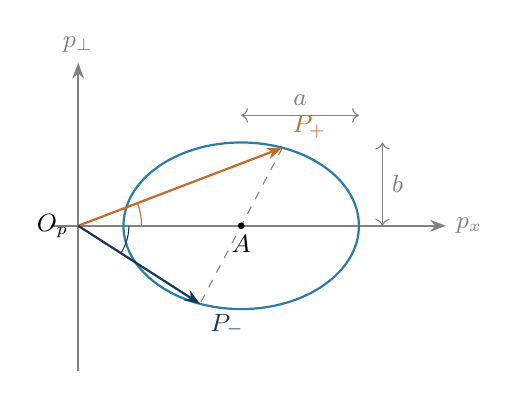
\begin{tikzpicture}[x=2.3cm,y=2.3cm]
  \draw[vec,gray] (-.15,0)--(2.03,0) node[right] {$p_x$};
  \draw[vec,gray] (0,-.8)--(0,.9) node[above] {$p_\perp$};
  \draw[field,thick] (.9,0) ellipse (.65 and .46);
  \draw[vec,force] (0,0)--(1.1275,.43091) node[above right] {$P_+$};
  \draw[vec,ink] (0,0)--(.6725,-.43091) node[below right] {$P_-$};
  \draw[helper] (1.1275,.43091)--(.6725,-.43091);
  \fill (.9,0) circle (1.2pt) node[below] {$A$};
  \draw[<->,gray] (.9,.61)--(1.55,.61) node[midway,above] {$a$};
  \draw[<->,gray] (1.68,0)--(1.68,.46) node[midway,right] {$b$};
  \draw[force] (.35,0) arc (0:20.92:.35);
  \draw[ink] (.28,0) arc (0:-32.65:.28);
  \node[left] at (0,0) {$O_p$};
\end{tikzpicture}
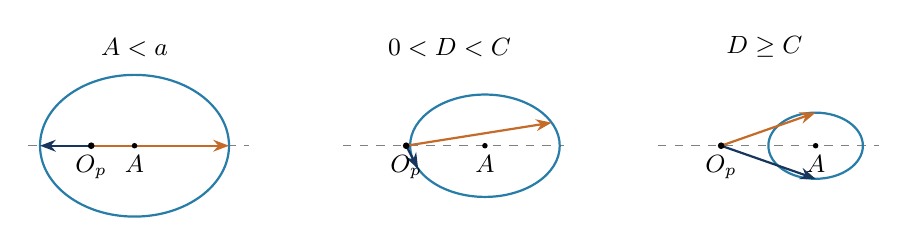
\begin{tikzpicture}
  \foreach \shift/\A/\aa/\bb/\uu/\label in {0/.55/1.2/.9/1/{$A<a$},4/1/0.95/0.65/0.89267855/{$0<D<C$},8/1.2/.6/.42/0/{$D\ge C$}}{
    \begin{scope}[xshift=\shift cm]
      \draw[helper] (-.8,0)--(2,0);
      \draw[field,thick] (\A,0) ellipse [x radius=\aa,y radius=\bb];
      \pgfmathsetmacro{\vv}{sqrt(1-\uu*\uu)}
      \draw[vec,force] (0,0)--({\A+\aa*\uu},{\bb*\vv});
      \draw[vec,ink] (0,0)--({\A-\aa*\uu},{-\bb*\vv});
      \fill (0,0) circle (1.2pt) node[below] {$O_p$};
      \fill (\A,0) circle (1pt) node[below] {$A$};
      \node at (.55,1.25) {\label};
    \end{scope}
  }
\end{tikzpicture}
\end{document}
